\documentclass[11pt]{article}

\usepackage[margin=1in]{geometry}
\usepackage{graphicx}
\usepackage{booktabs}
\usepackage{longtable}
\usepackage{array}
\usepackage{float}
\usepackage{hyperref}
\usepackage{amsmath}
\usepackage{caption}

\graphicspath{{../Results/images/}}

\title{Heterogeneous LLM-Based Trading Agents in Continuous Double-Auction Markets: A Controlled Evaluation Against Adaptive Benchmarks in ABIDES}
\author{Nguyen Quy Tu \and Nguyen Minh Nghia}
\date{Progress Report, June 2026}

\begin{document}
\maketitle

\begin{abstract}
Continuous double auctions (CDAs) are the dominant trading mechanism in real equity and commodity markets, and recent work shows that large language models (LLMs) can act as plausible trading agents within them. This project evaluates a locally hosted open-source LLM, Gemma 3 4B Instruct, as a trading agent inside ABIDES, a high-fidelity discrete-event market simulator. The study compares the LLM against adaptive and traditional algorithmic benchmarks under controlled ablations of prompt structure, memory, information access, latency, regime shocks, and inter-agent communication.

This progress report preserves the original experimental plan while updating the preliminary evidence. Experiments 1 and 2 established a functioning ABIDES baseline and showed that inserting a naive LLM trader greatly increases trading activity and market instability while producing severe LLM losses. Experiment 3 then isolated prompt structure and found that unstructured chain-of-thought is harmful for the small model, while structured evidence-grounded reasoning improves both compliance and PnL. Experiment 4 isolated memory design and found that memory can improve trading outcomes, but its effect depends strongly on whether the prompt allows reasoning and whether execution history is summarized or appended raw. Because Experiments 5--8 have not yet been carried out, the empirical section remains preliminary.
\end{abstract}

\section{Background and Motivation}

Continuous double auctions, in which buyers and sellers continuously submit orders to a central limit order book, underpin real-world equity and commodity exchanges. Open-source simulators such as the Bristol Stock Exchange (BSE), ABIDES, and PyMarketSim make it possible to study market microstructure under controlled, repeatable conditions that would be impossible to obtain with human participants.

Recent literature establishes the viability of LLMs as trading agents within such simulations. Lopez-Lira (2025) demonstrates that LLM agents can follow strategy instructions, occupy roles such as value investor or momentum trader, and reproduce market phenomena including price discovery, bubbles, underreaction, and liquidity provision. Agrawal et al. (2025) study LLM sellers in a CDA and find that direct communication increases collusive tendencies, motivating a dedicated communication experiment.

Important questions remain open. Most published work centers on large proprietary or API-hosted models. The behavior of small, locally hosted open-source models under tight resource and latency budgets is less understood. The interaction between prompt design, memory design, information access, and decision latency has also not been systematically ablated within one high-fidelity environment. This study addresses those gaps by evaluating a single local model in ABIDES across controlled experimental conditions.

\section{Simulator Selection: BSE versus ABIDES}

The simulator choice is consequential because latency and communication experiments require capabilities that not all CDA simulators provide. Table~\ref{tab:simulators} summarizes the comparison.

\begin{table}[H]
\centering
\caption{Comparison of BSE and ABIDES}
\label{tab:simulators}
\begin{tabular}{p{0.22\linewidth}p{0.34\linewidth}p{0.34\linewidth}}
\toprule
Dimension & BSE & ABIDES \\
\midrule
Architecture & Single-script, sequential order processing & Discrete-event, message-passing engine modeled on exchange protocols \\
Latency model & No exchange or network latency & Configurable pairwise latency and agent computation delays \\
Communication & No private inter-agent messaging & Standardized messages and private agent communication \\
Adaptive agents & GVWY, SHVR, ZIC, ZIP, AA, GDX & ZI, HBL, value, momentum, market-maker, and noise agents \\
Value process & Exogenous customer schedules & Dynamic mean-reverting common-value process \\
Best suited to & Teaching and rapid strategy prototyping & High-fidelity microstructure, latency, and communication studies \\
\bottomrule
\end{tabular}
\end{table}

ABIDES is required for the core study for five reasons. First, Experiment 6 requires a latency model, which BSE does not provide. Second, Experiment 8 requires private message-based communication. Third, ABIDES includes Heuristic Belief Learning (HBL), a native adaptive benchmark. Fourth, its dynamic fundamental value process supports price-versus-equilibrium analysis and shock-response experiments. Fifth, the ABIDES ecosystem supports structured, reproducible market runs.

\section{Agent Design and Architecture}

\subsection{Local LLM Integration}

The LLM trader uses Gemma 3 4B Instruct served locally through Ollama. The endpoint is OpenAI-compatible at \texttt{http://localhost:11434/v1}, and ABIDES queries it through the standard \texttt{openai} Python client. Local hosting removes API cost and uncontrolled network latency. It also makes the planned latency experiment more interpretable because artificial delays can be introduced deliberately.

The local hardware constraint is a 4GB VRAM GPU. Gemma 3 4B is therefore used with 4-bit quantization through Ollama. This keeps the model and context within GPU memory while leaving enough room for compact state descriptions, prompt scaffolds, and memory summaries.

\subsection{Background and Benchmark Agents}

The primary adaptive benchmark is the HBL agent native to ABIDES, based on Gjerstad and Dickhaut's belief-learning trader. HBL estimates the probability that a candidate bid or ask will transact from recent order-book history, then quotes to maximize expected surplus. Because it is order-book-aware and adaptive, HBL is a more demanding benchmark than zero-intelligence trading. ZI, value, and momentum agents are used to supply liquidity, noise, and additional strategy diversity.

\subsection{LLM Output and Memory}

The LLM agent converts the current market state into a compact prompt containing top-of-book prices, recent market variables, position, and cash. The output is parsed into a trading action: buy, sell, or hold, with price and quantity when applicable. Later experiments modify the prompt scaffold, memory horizon, information access, and latency while holding the simulator and background population fixed.

For memory ablation, the implemented memory modes are: no history, last 5 events, last 20 events, and rolling session summary. Additional diagnostic variants either allow a one-sentence rationale or add successful fills to the remembered event stream.

\section{Experimental Methodology}

All experiments run locally in ABIDES. Each reported run uses exactly 10 agents: one LLM trader and nine traditional background agents unless otherwise specified. The current completed experiments use seed 12345. The target for publishable conclusions remains replication across at least 10 seeds per condition, with results reported as means and dispersion.

The planned experiment suite is:

\begin{enumerate}
    \item \textbf{Baseline Market Reproduction.} Ten traditional agents validate that the environment produces sensible spreads, continuous volume, and price discovery.
    \item \textbf{LLM in the Market vs. Background.} Insert one LLM trader into the traditional background and compare spreads, price tracking, and PnL.
    \item \textbf{Prompt Ablation.} Vary the prompt across minimal, unstructured reasoning, structured reasoning, evidence-grounded reasoning, and JSON-envelope variants.
    \item \textbf{Memory Ablation.} Vary the single LLM's memory across no history, last 5 events, last 20 events, and rolling summary.
    \item \textbf{Information-Access Ablation.} Vary the market view across top-of-book, visible LOB, recent trades, and inventory/PnL enriched state.
    \item \textbf{Latency Sensitivity.} Add artificial decision delays through the ABIDES latency model.
    \item \textbf{Shock-Response Market.} Introduce a mid-session change in fundamental value or supply-demand regime.
    \item \textbf{Communication and Collusion.} Use two same-side LLM traders and vary private messaging before quoting.
\end{enumerate}

\section{Evaluation Metrics}

Evaluation focuses on three interpretable metric families.

\textbf{Bid-ask spread} measures how agents adapt their quotes. A wide spread indicates disagreement or poor adjustment; a narrowing spread indicates improved quote adaptation and market quality.

\textbf{Price versus equilibrium} compares the realized mid-price and transaction prices against the fundamental value generated by ABIDES. This measures whether the market discovers the underlying value process or drifts away from it.

\textbf{Profit and loss (PnL)} answers whether the LLM trader is actually competitive. We report mark-to-market PnL and rank among the 10 agents. In communication experiments, seller-side PnL and surplus will also serve as indicators of coordination or collusion.

Supporting diagnostics include parse failures, fallback holds, deliberate holds, token usage, reasoning-binding rate, and qualitative inspection of LLM reasoning traces.

\section{Preliminary Results}

Experiments 1--4 have been completed as single-seed or diagnostic runs. These results should be read as preliminary: they establish the engineering pipeline and reveal plausible mechanisms, but they are not yet statistically confirmed. Experiments 5--8 remain planned future work.

\subsection{Experiment 1: Traditional Baseline}

Experiment 1 validates the ABIDES market without an LLM trader. The configuration contains 10 traditional agents: four zero-intelligence agents, three HBL agents, two value agents, and one momentum agent. The two-hour session runs successfully and produces continuous trading.

\begin{figure}[H]
\centering
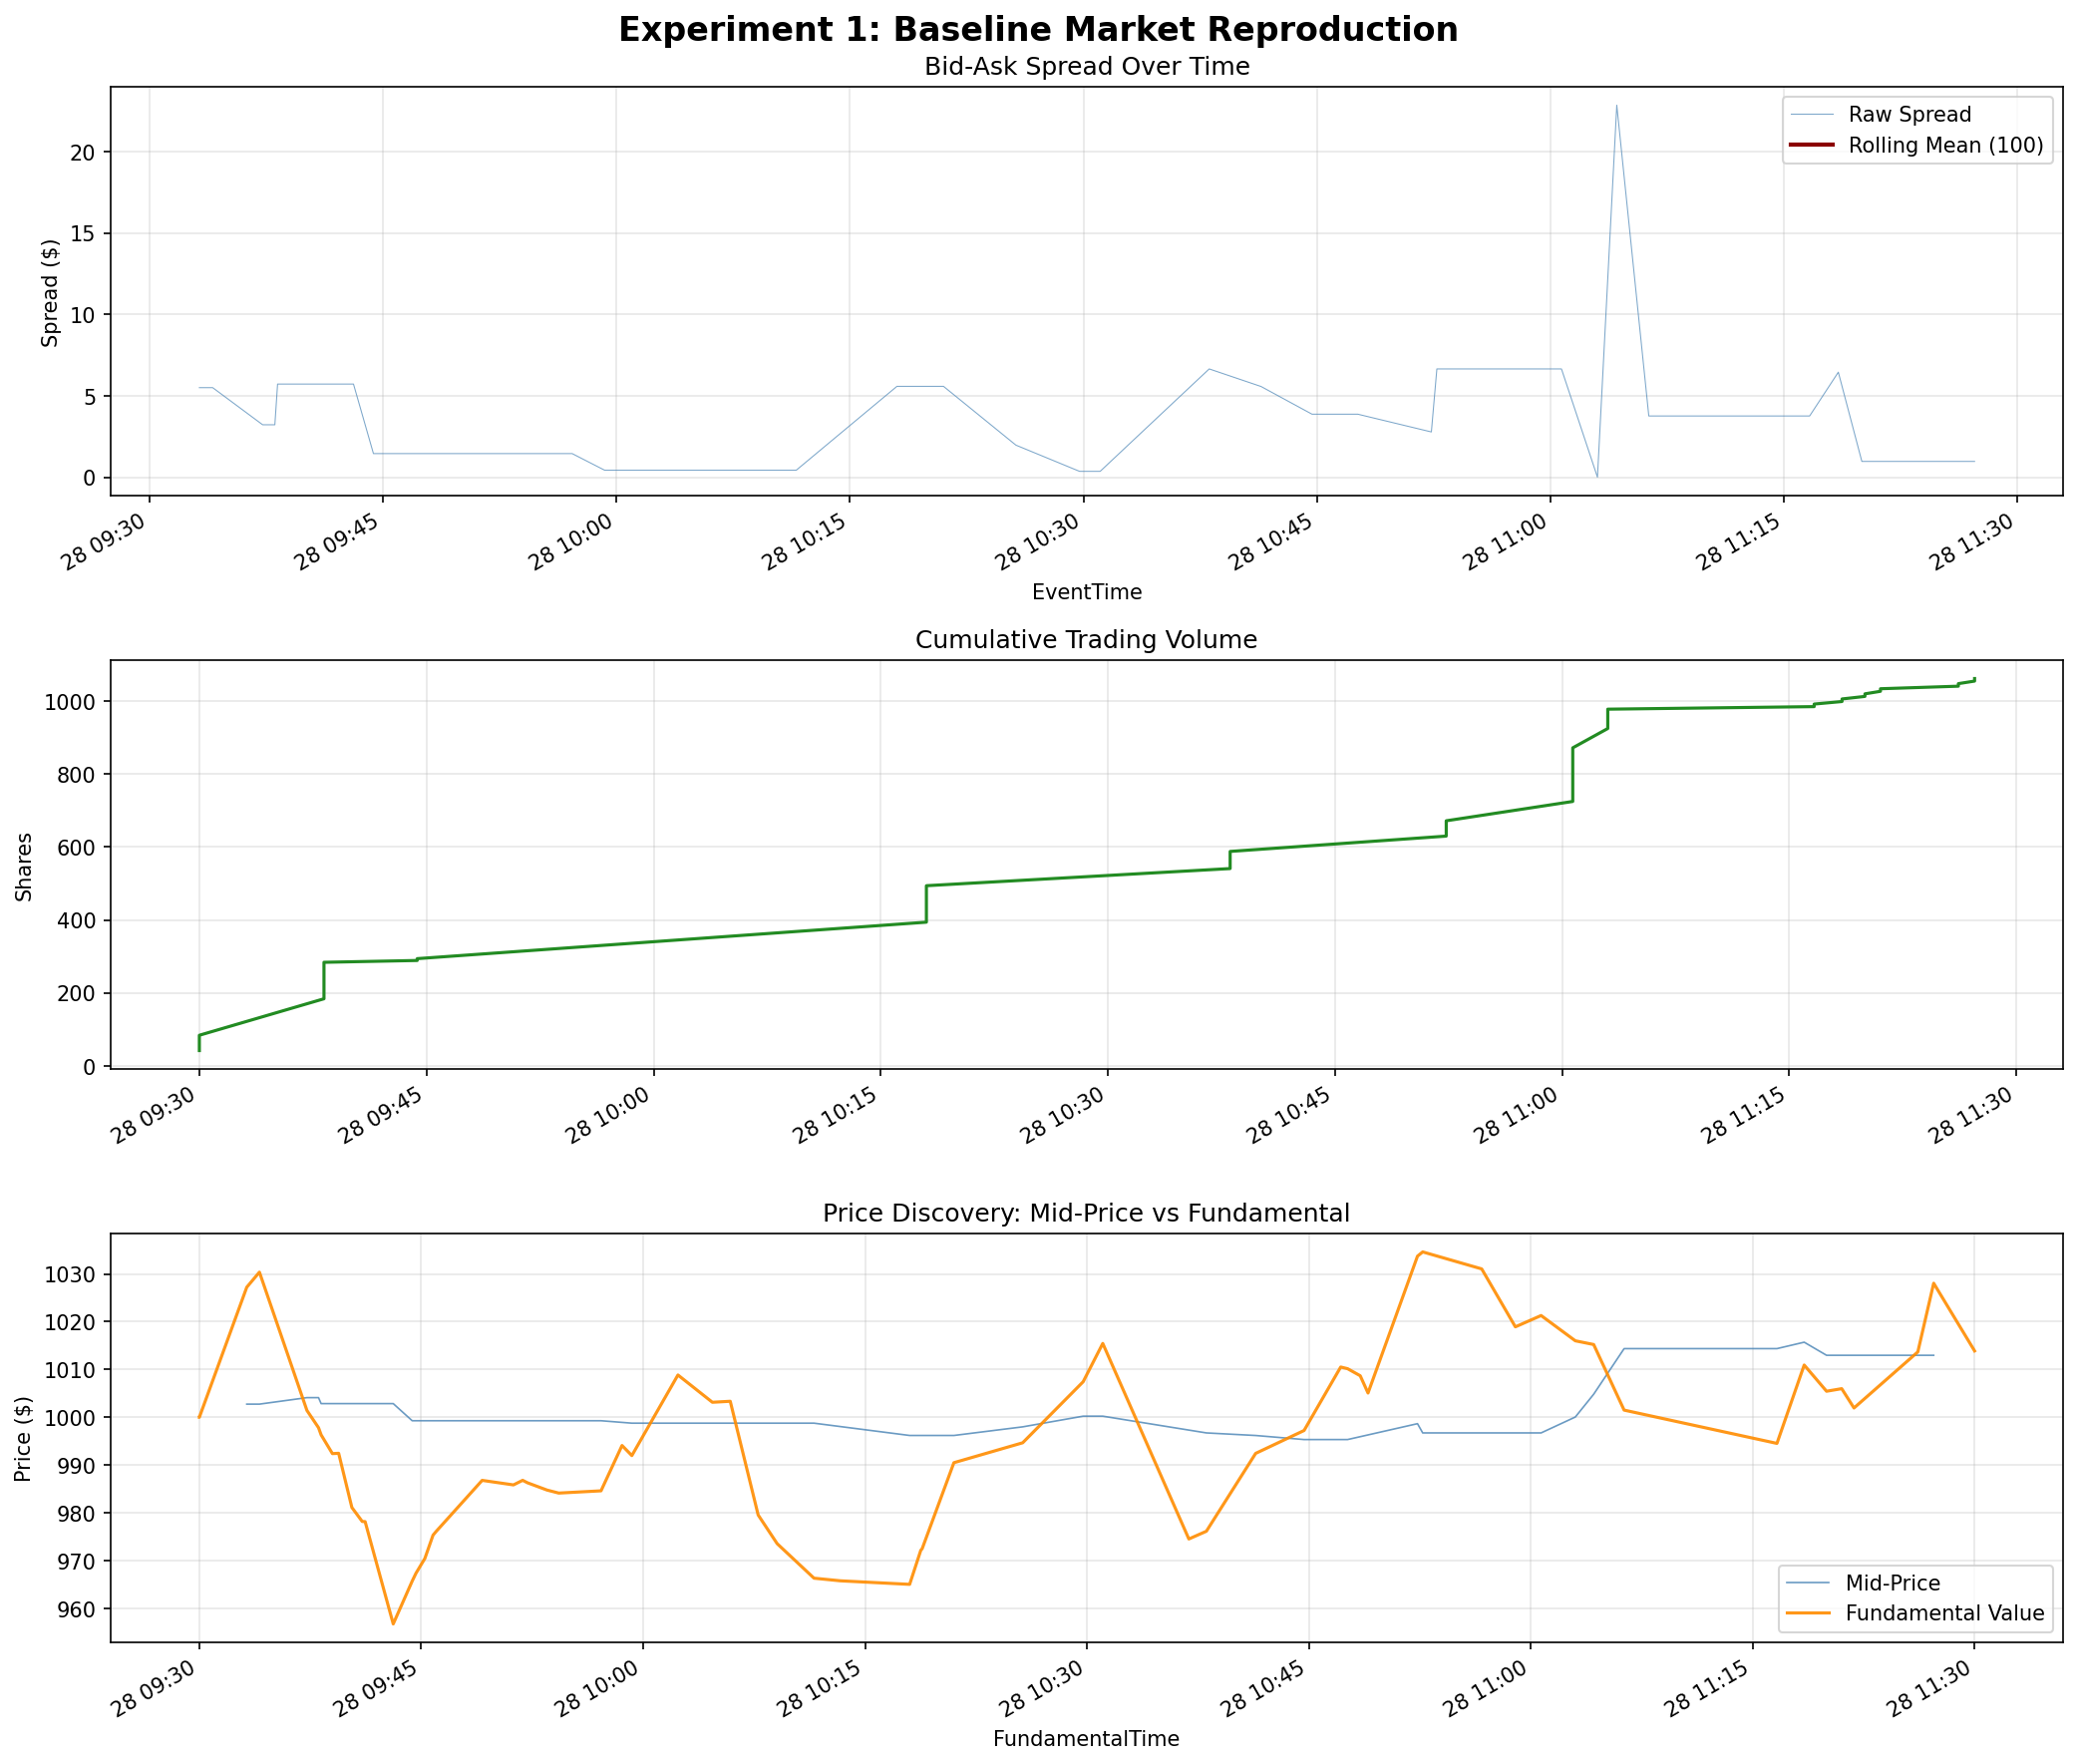
\includegraphics[width=0.92\linewidth]{exp1_baseline_analysis.png}
\caption{Experiment 1 traditional-agent baseline: spread, cumulative volume, and mid-price versus fundamental value.}
\label{fig:exp1}
\end{figure}

\begin{table}[H]
\centering
\caption{Experiment 1 market summary}
\label{tab:exp1-summary}
\begin{tabular}{lr}
\toprule
Metric & Value \\
\midrule
Mean spread & \$3.30 \\
Median spread & \$1.71 \\
Total volume & 1,062 shares \\
Executions & 30 \\
Mean mid-price & \$1,002.62 \\
Mid-price standard deviation & \$6.44 \\
\bottomrule
\end{tabular}
\end{table}

The market is calm and orderly. Spreads stabilize after an initial transient period, volume accumulates steadily, and the mid-price tracks the fundamental value only loosely but without extreme instability. HBL agents earn the largest aggregate profit, while ZI agents lose money overall, matching the expected advantage of adaptive order-book-aware strategies over random trading.

\subsection{Experiment 2: Naive LLM-Inclusive Market}

Experiment 2 replaces one traditional agent with a Gemma 3 4B LLM trader using a strict JSON decision prompt. All other market parameters remain aligned with Experiment 1.

\begin{figure}[H]
\centering
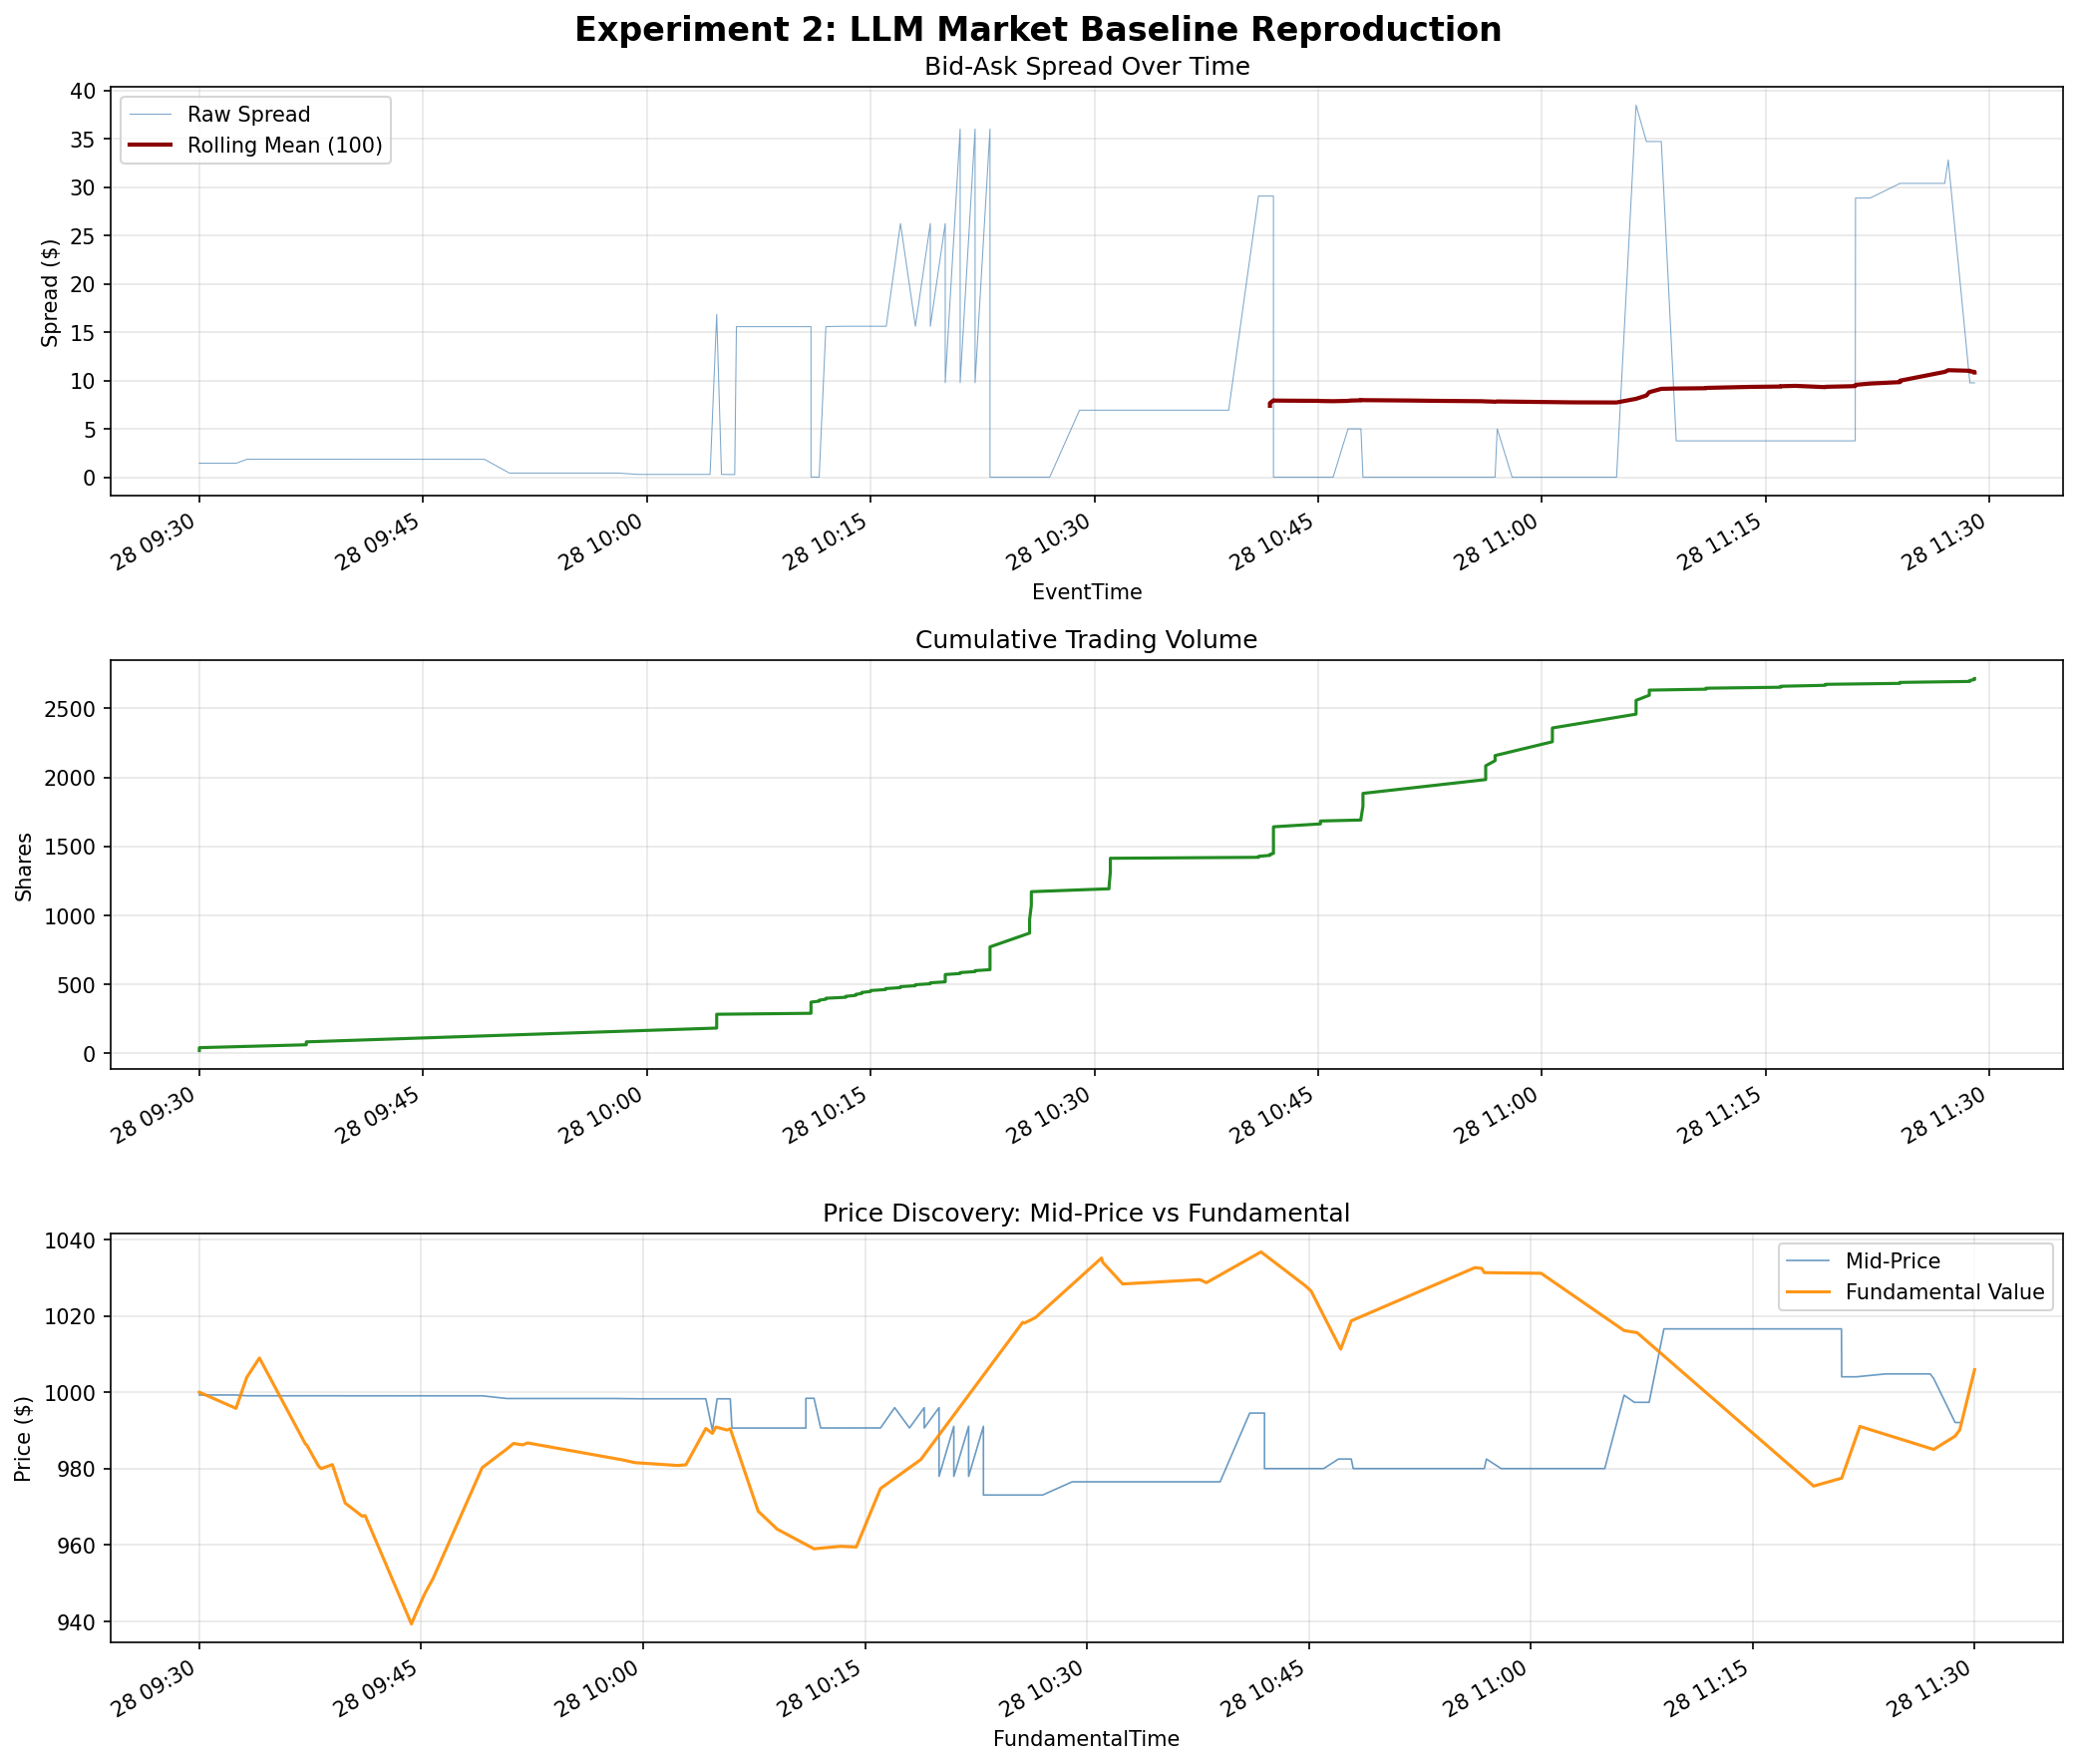
\includegraphics[width=0.92\linewidth]{exp2_llm_baseline_analysis.png}
\caption{Experiment 2 LLM-inclusive market: spread, cumulative volume, and mid-price versus fundamental value.}
\label{fig:exp2}
\end{figure}

\begin{table}[H]
\centering
\caption{Experiment 2 market summary}
\label{tab:exp2-summary}
\begin{tabular}{lrr}
\toprule
Metric & Experiment 1 & Experiment 2 \\
\midrule
Mean spread & \$3.30 & \$8.15 \\
Total volume & 1,062 & 2,716 \\
Executions & 30 & 86 \\
Mean mid-price & \$1,002.62 & \$992.42 \\
Mid-price standard deviation & \$6.44 & \$11.71 \\
\bottomrule
\end{tabular}
\end{table}

The naive LLM trader sharply disrupts the market. Volume rises by more than 2.5 times, spreads become wider and spikier, and mid-price volatility increases. The LLM trader performs very poorly, with PnL of \(-\$16{,}106.42\), while HBL agents earn strongly positive aggregate profits. This indicates that the base local model has no reliable financial intuition under the naive prompt and that background agents can exploit its poor order placement.

\subsection{Experiment 3: Prompt-Level Reasoning Ablation}

Experiment 3 asks whether better prompt scaffolding can improve the LLM trader while holding non-prompt parameters fixed. The arms are Minimal-Raw, R1 Open CoT, R2 Structured CoT, R3 Evidence-Grounding, and a structured JSON envelope equivalent to R3.

\begin{figure}[H]
\centering
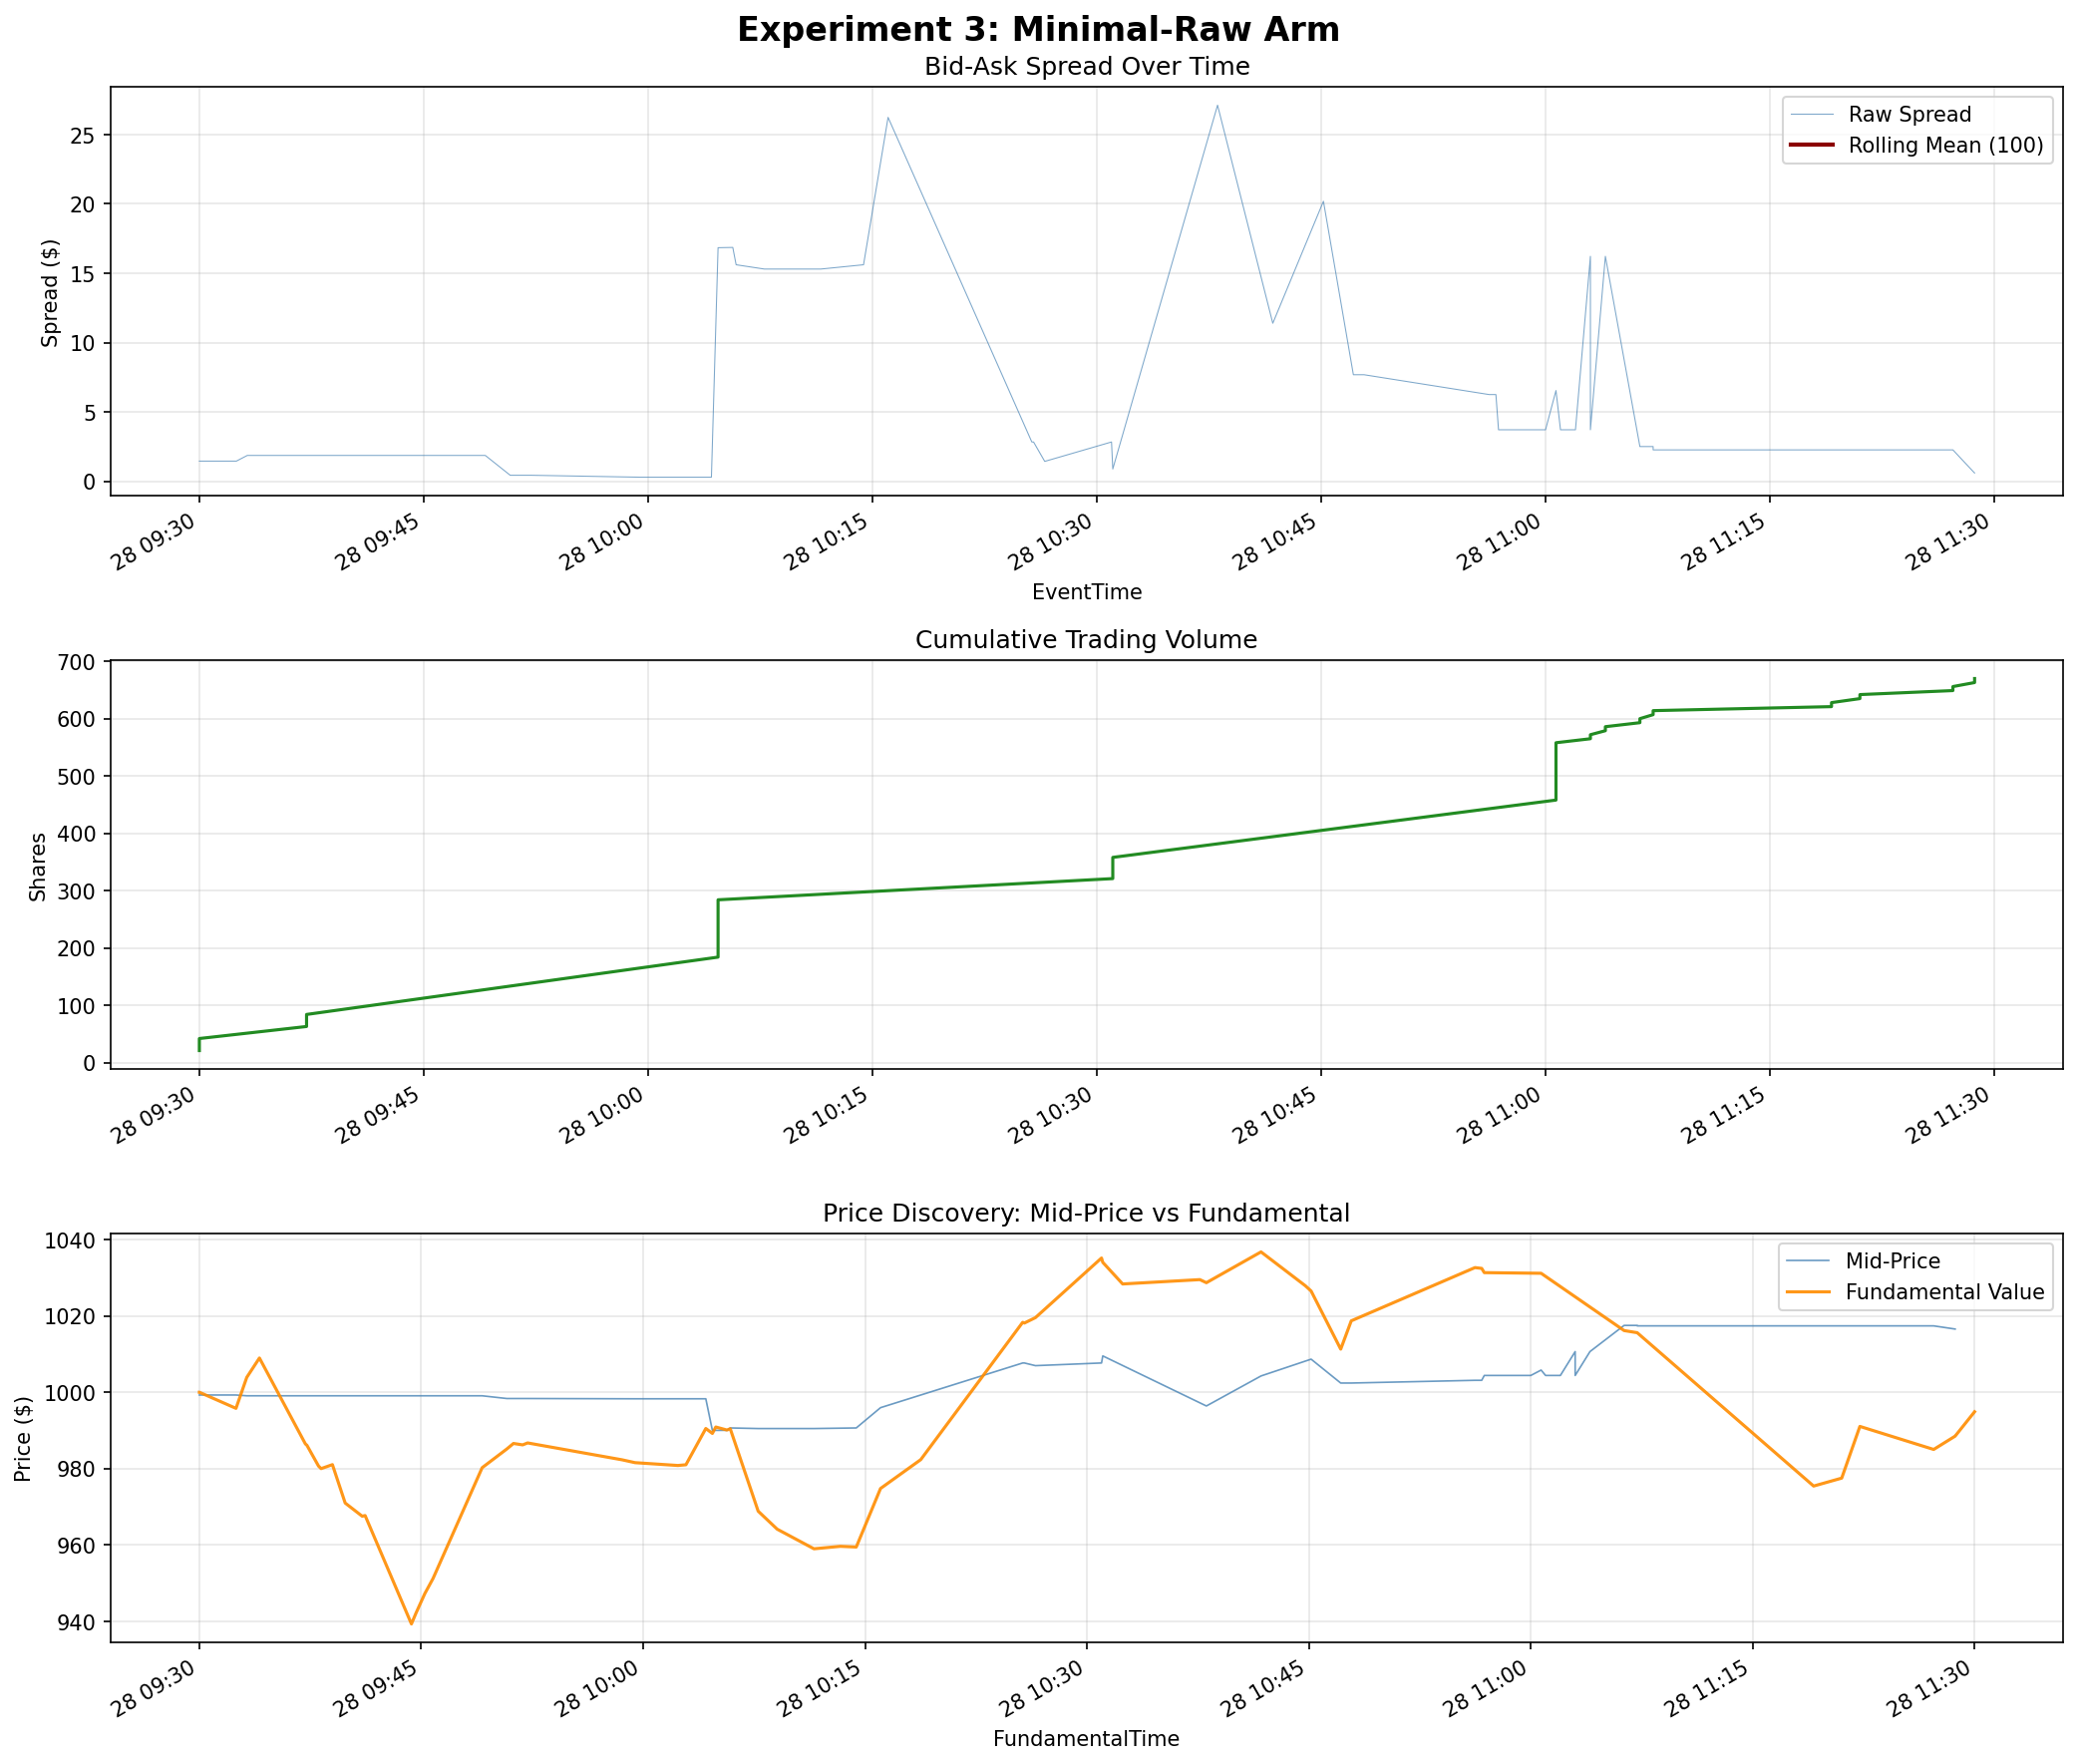
\includegraphics[width=0.86\linewidth]{result_exp3_minimal_raw.png}
\caption{Experiment 3 Minimal-Raw market dynamics.}
\label{fig:exp3-minimal}
\end{figure}

\begin{figure}[H]
\centering
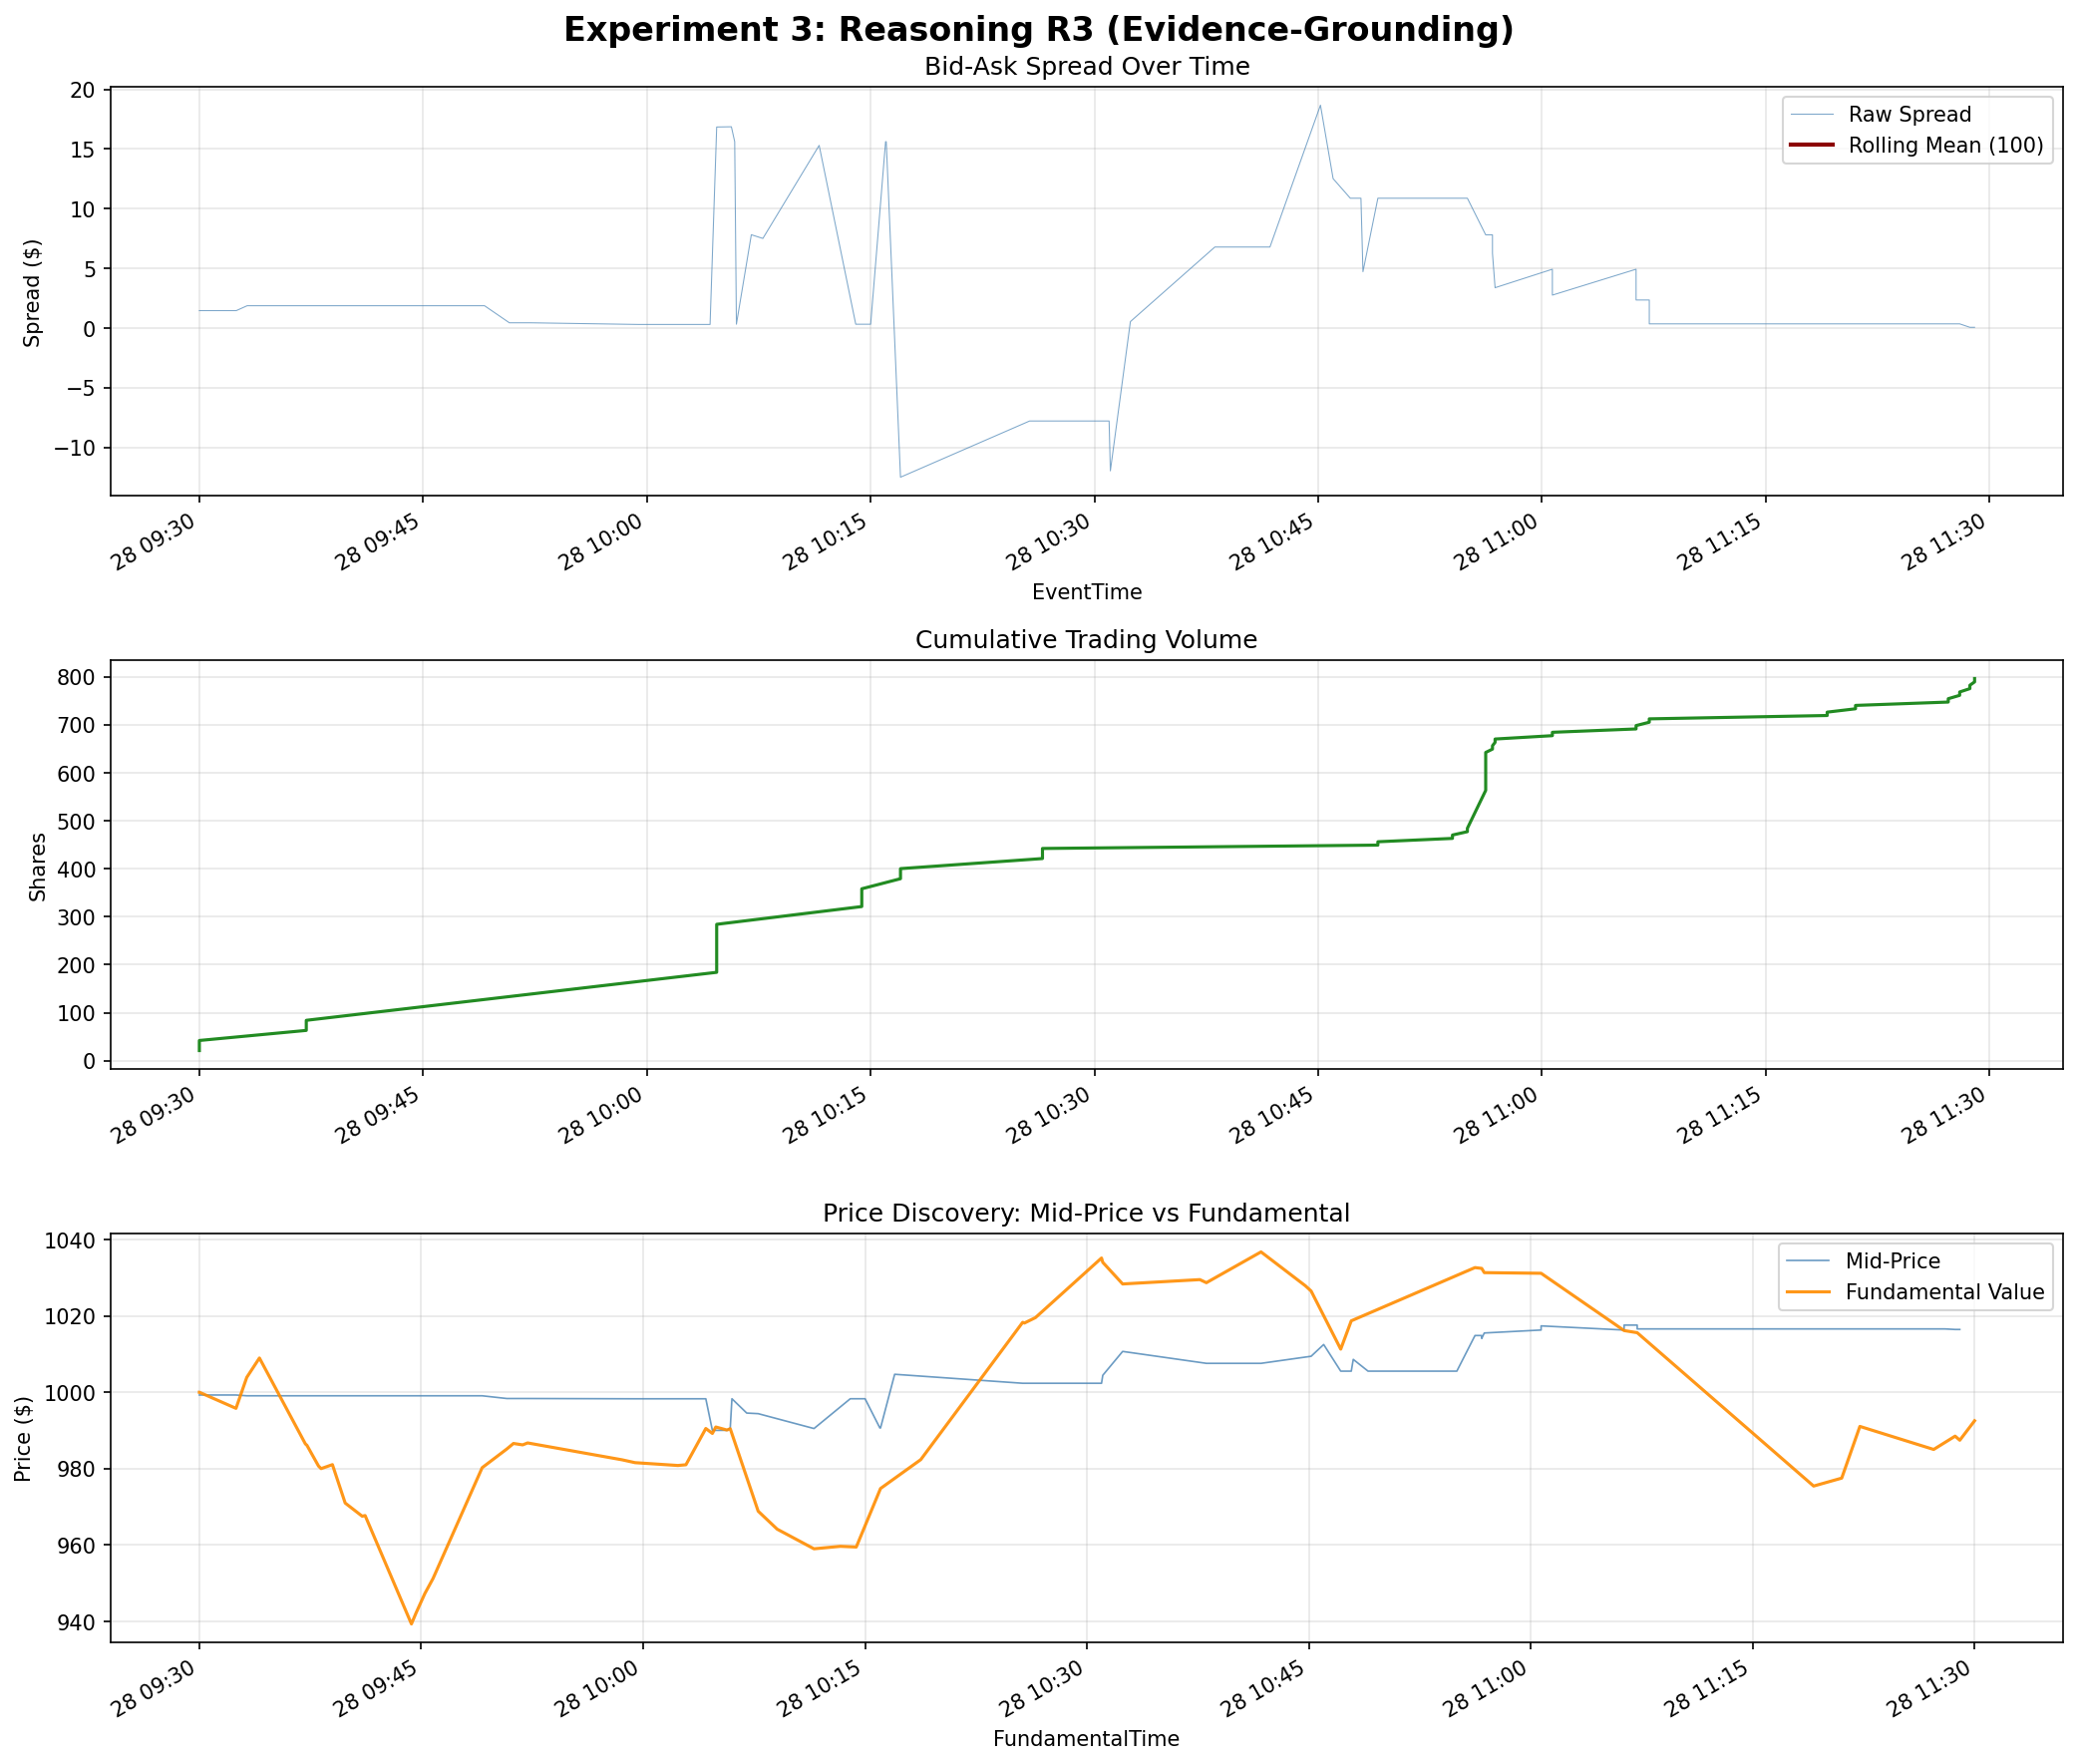
\includegraphics[width=0.86\linewidth]{exp3_reasoning_r3_analysis.png}
\caption{Experiment 3 R3 evidence-grounded reasoning market dynamics.}
\label{fig:exp3-r3}
\end{figure}

\begin{table}[H]
\centering
\caption{Experiment 3 LLM prompt ablation summary}
\label{tab:exp3}
\begin{tabular}{lrrrrr}
\toprule
Metric & Minimal & R1 & R2 & R3 & JSON \\
\midrule
Parse failures & 0/119 & 19/119 & 0/119 & 0/119 & 0/119 \\
Median tokens & 5 & 62 & 88 & 122 & 103 \\
Verify citation rate & -- & -- & -- & 119/119 & 2/119 \\
LLM PnL & \$0.00 & \(-\$5{,}362.67\) & \$148.05 & \$793.92 & \(-\$889.34\) \\
Rank of 10 & 6th & 10th & 3rd & 2nd & 9th \\
\bottomrule
\end{tabular}
\end{table}

The central finding is that unstructured reasoning is harmful for this small local model. R1's instruction to think step by step introduces 19 parse failures and leads to a severe loss. Structured tags in R2 restore perfect parse compliance and produce marginally positive PnL. Adding a \texttt{[VERIFY]} step in R3 improves PnL to \$793.92 and ranks the LLM second among 10 agents. The model appears to benefit most not from more text, but from forced grounding in concrete state values.

The JSON-envelope variant is especially important. It preserves perfect formatting but degrades decision quality: the verify citation rate falls from 100\% in plain-text R3 to 1.7\%, and PnL falls to \(-\$889.34\). This supports the hypothesis that strict syntactic envelopes consume useful reasoning capacity in a small model. Across all prompt arms, deliberate hold count remains zero; the model treats nearly every wakeup as a command to trade.

\subsection{Experiment 4: Memory Ablation}

Experiment 4 isolates memory design. The primary condition fixes the prompt to decision-only JSON with no reasoning, so the treatment variable is memory rather than prompt structure. Two diagnostic variants were also run: one that allows a one-sentence reasoning field and one that adds successful fills to the memory source.

\begin{figure}[H]
\centering
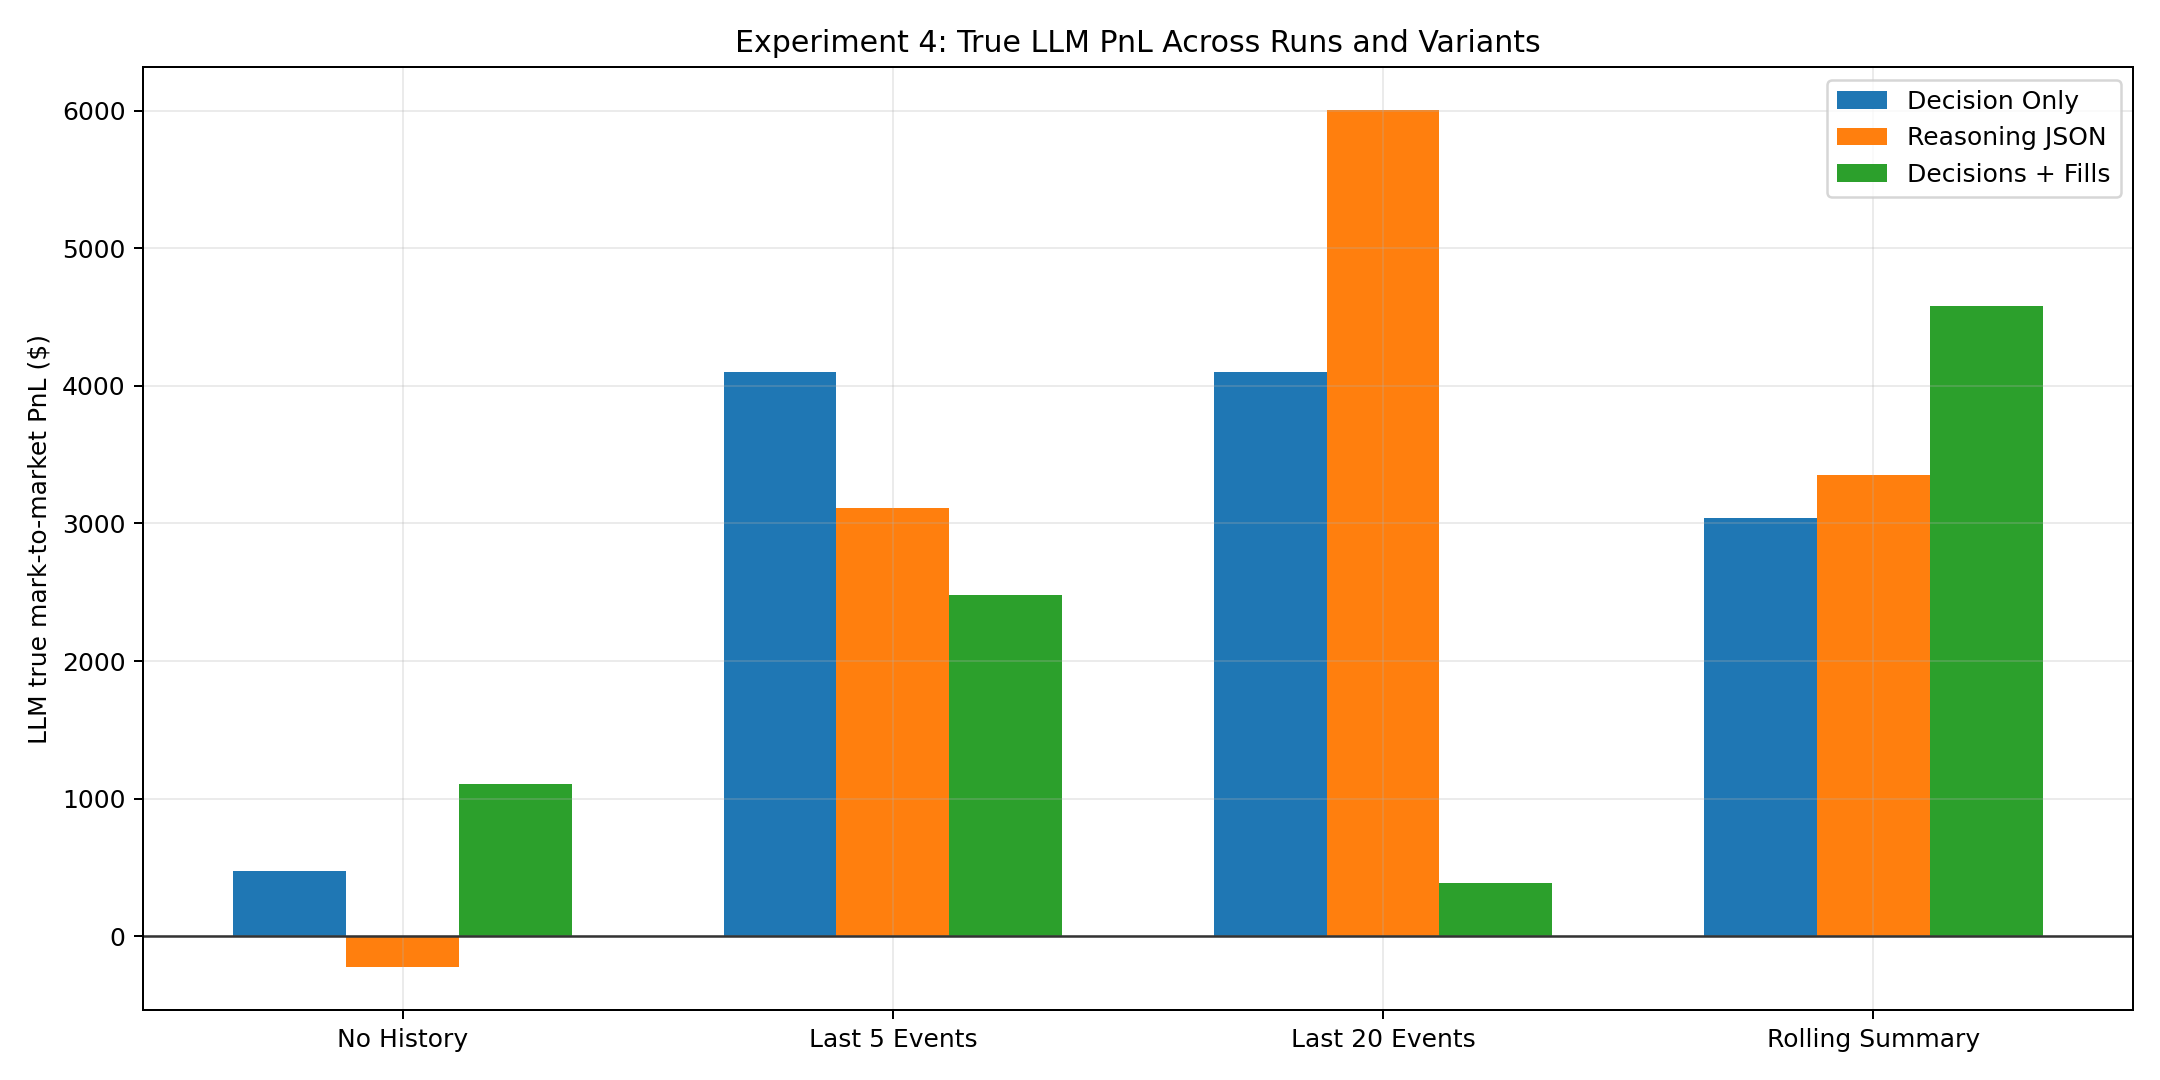
\includegraphics[width=0.92\linewidth]{exp4_full_pnl_comparison.png}
\caption{Experiment 4 true LLM mark-to-market PnL across memory arms and diagnostic variants.}
\label{fig:exp4-pnl}
\end{figure}

\begin{figure}[H]
\centering
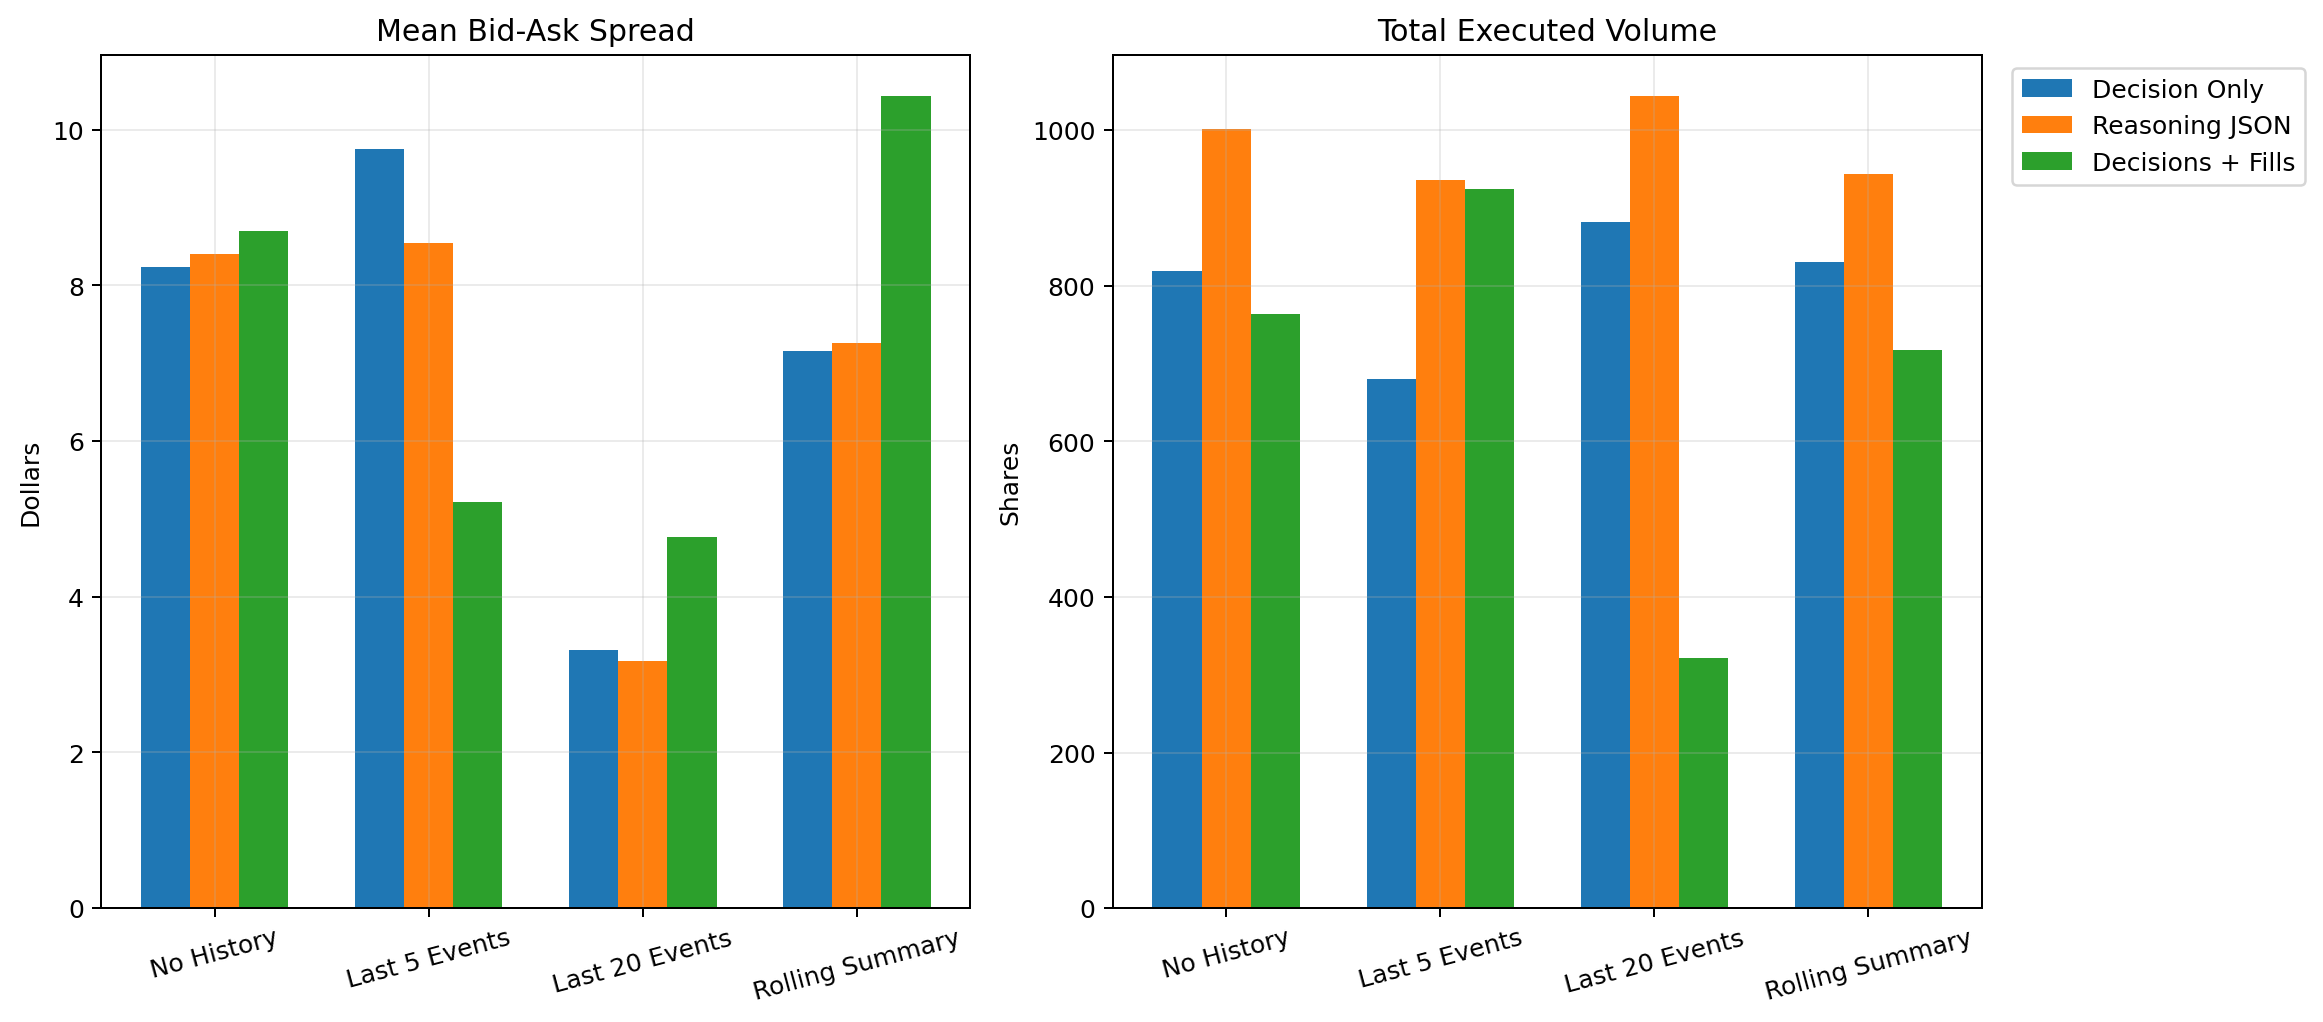
\includegraphics[width=0.92\linewidth]{exp4_full_market_comparison.png}
\caption{Experiment 4 market comparison across memory arms and diagnostic variants.}
\label{fig:exp4-market}
\end{figure}

The aggregate market comparison in Figure~\ref{fig:exp4-market} reports spread and volume, but the price-versus-equilibrium metric is inspected through the per-run market-dynamics plots below. In each plot, the third panel overlays the realized mid-price against the ABIDES fundamental value. These figures therefore provide the current qualitative price-discovery evidence for Experiment 4. A numeric tracking-error metric, such as mid-price RMSE against the fundamental value, is not yet included and remains a next-step measurement.

\begin{figure}[H]
\centering
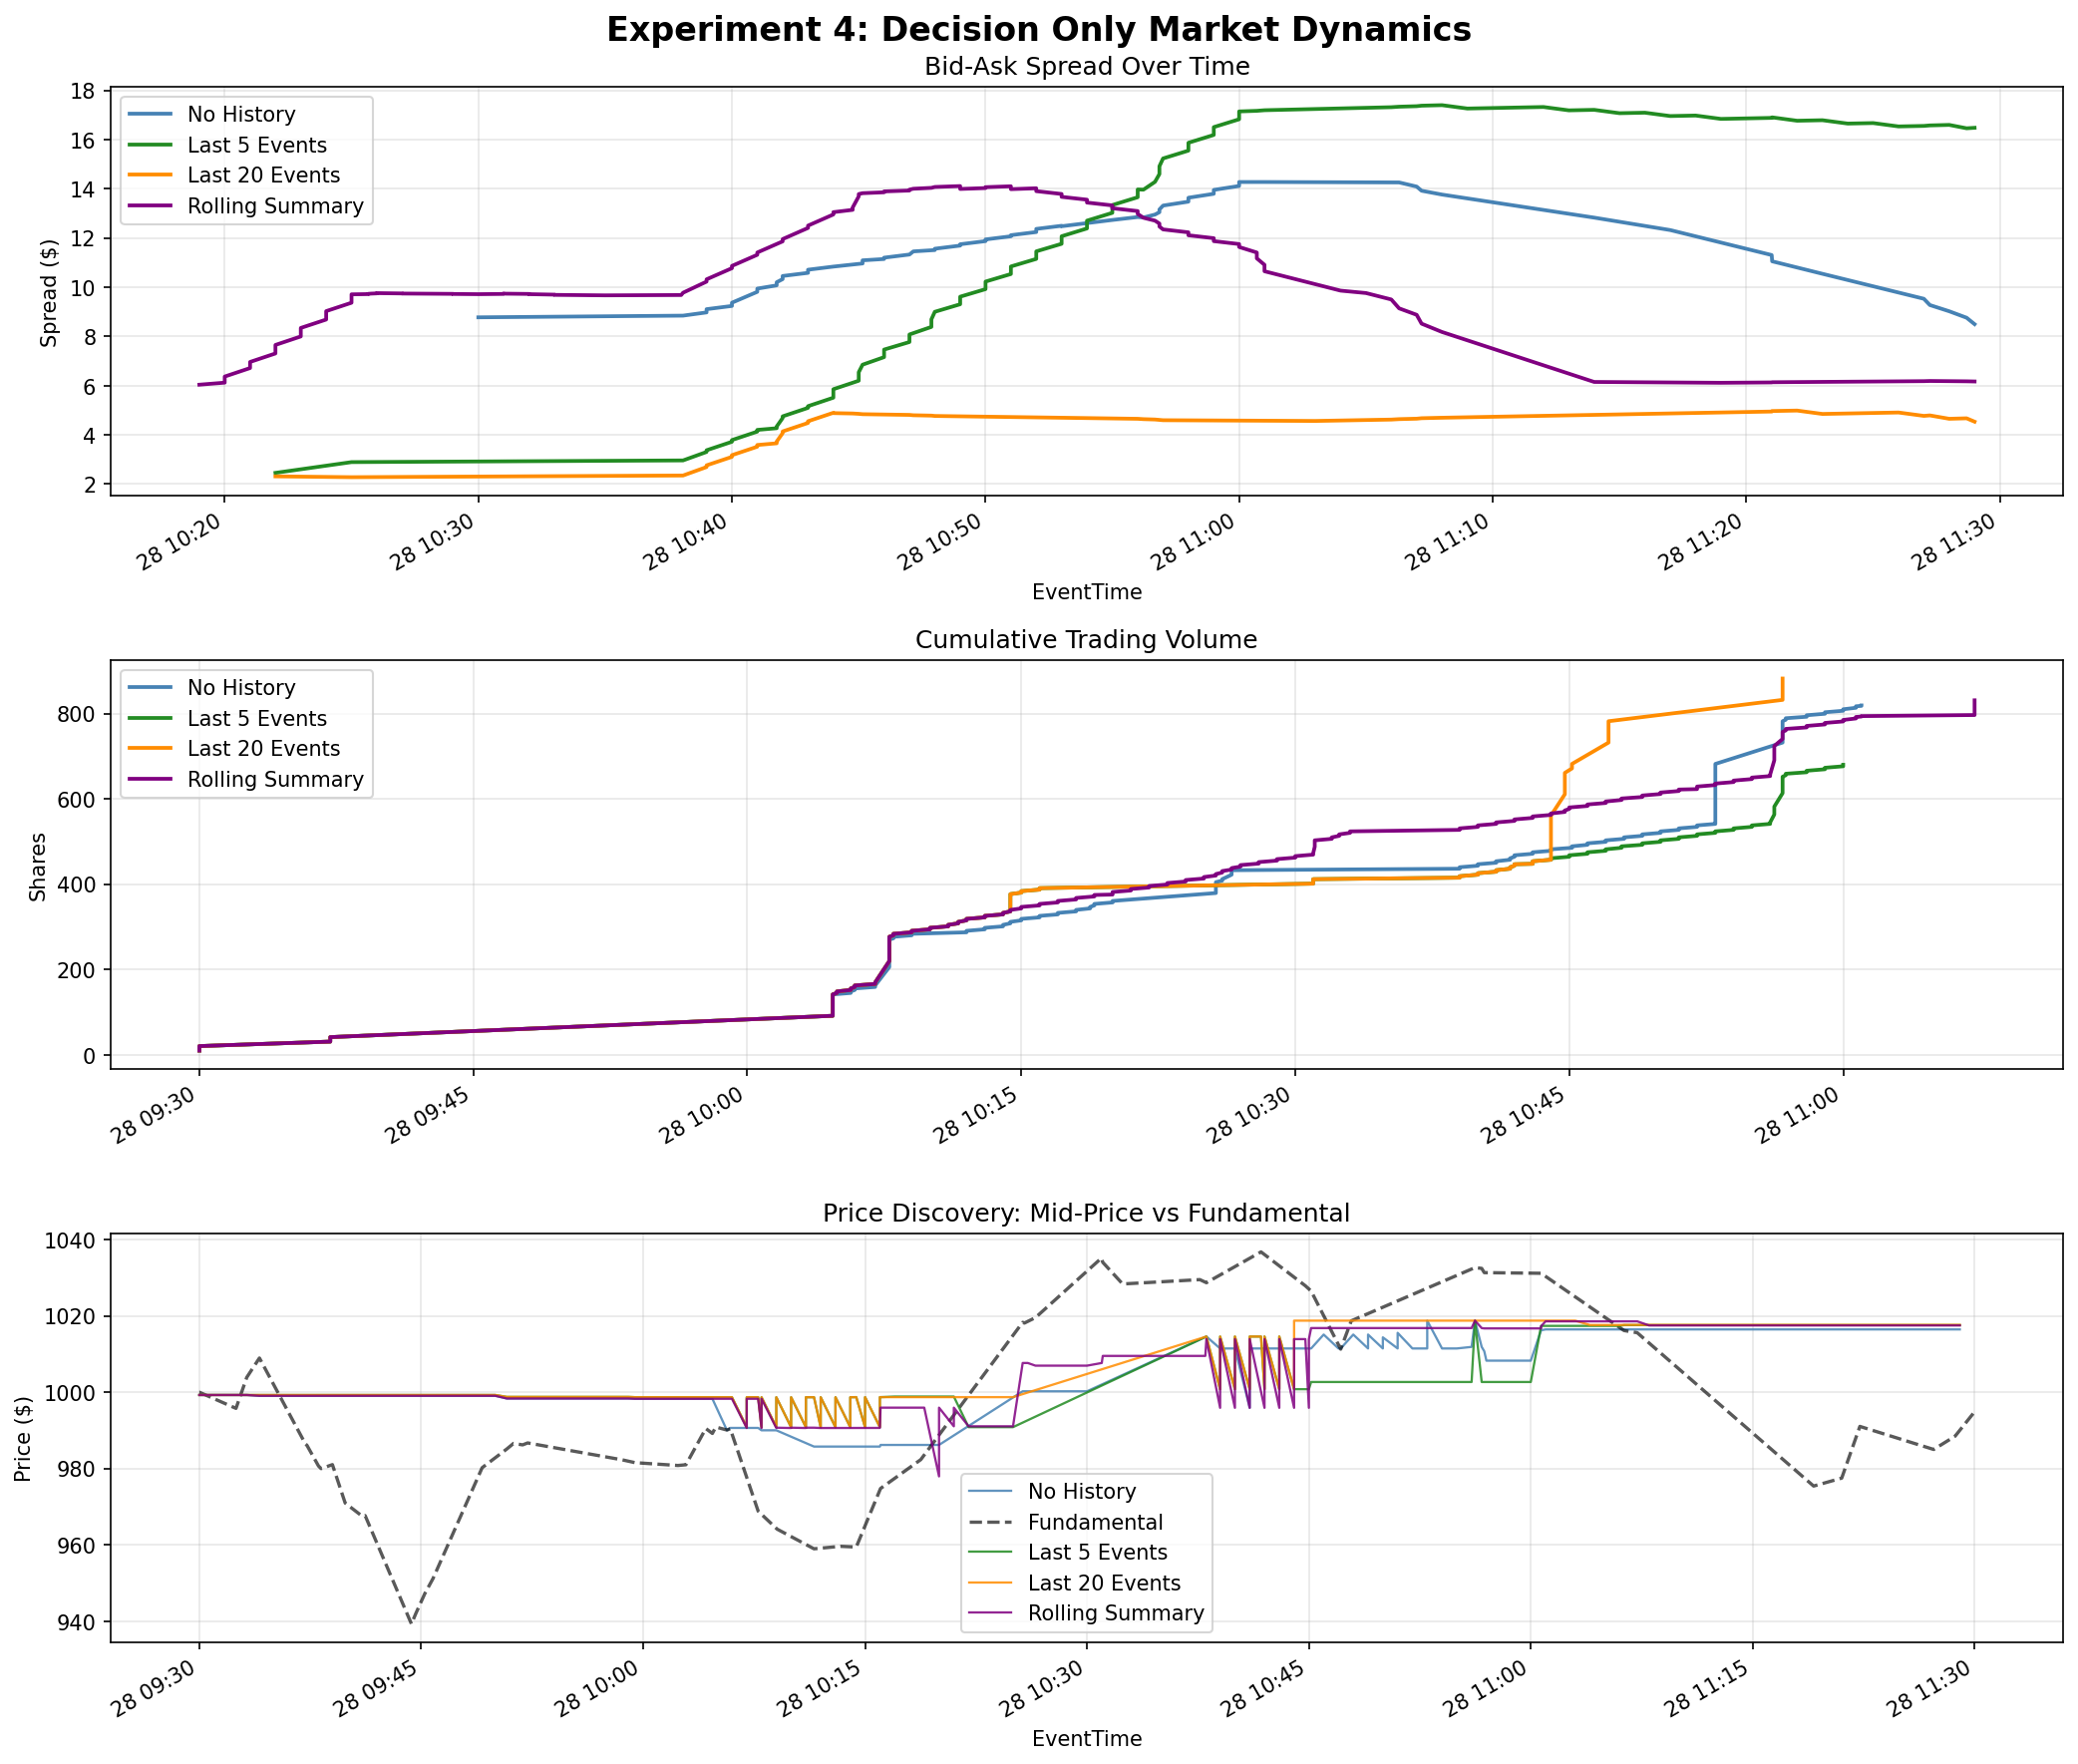
\includegraphics[width=0.92\linewidth]{exp4_rerun_decision_only_analysis.png}
\caption{Experiment 4 decision-only memory ablation: spread, cumulative volume, and mid-price versus fundamental value.}
\label{fig:exp4-decision-only}
\end{figure}

\begin{figure}[H]
\centering
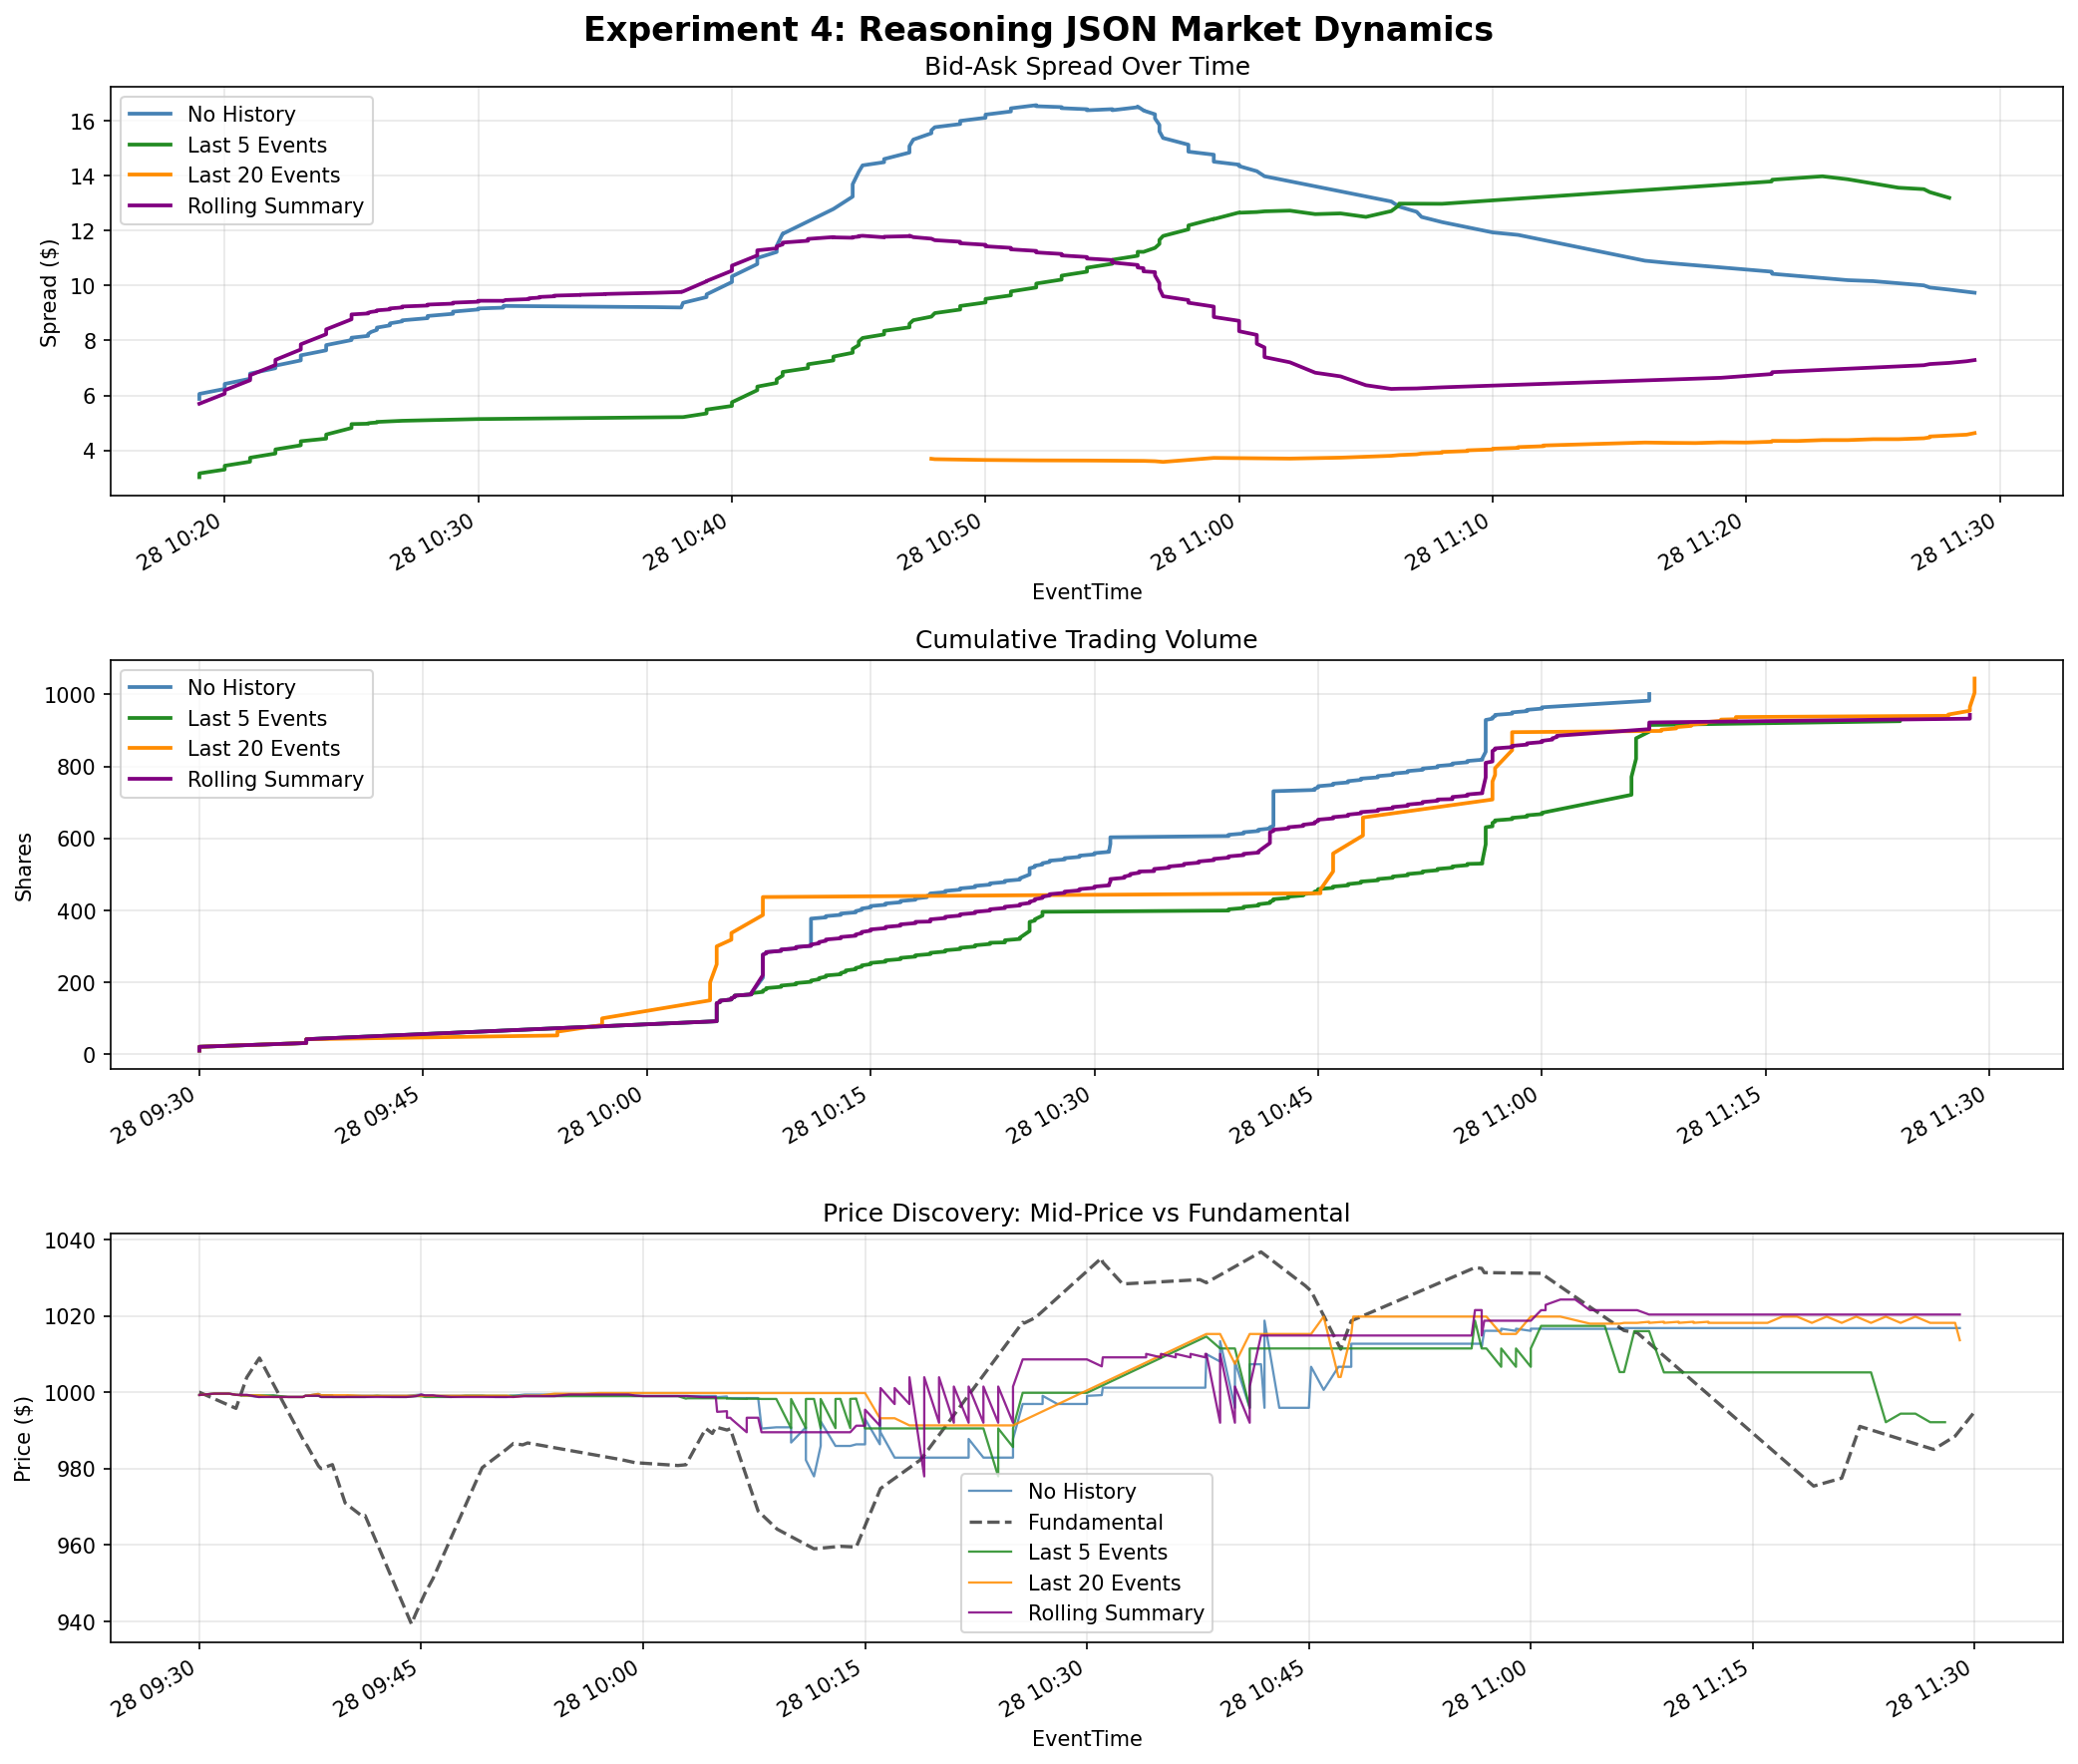
\includegraphics[width=0.92\linewidth]{exp4_reasoning_json_analysis.png}
\caption{Experiment 4 reasoning-JSON diagnostic: spread, cumulative volume, and mid-price versus fundamental value.}
\label{fig:exp4-reasoning}
\end{figure}

\begin{figure}[H]
\centering
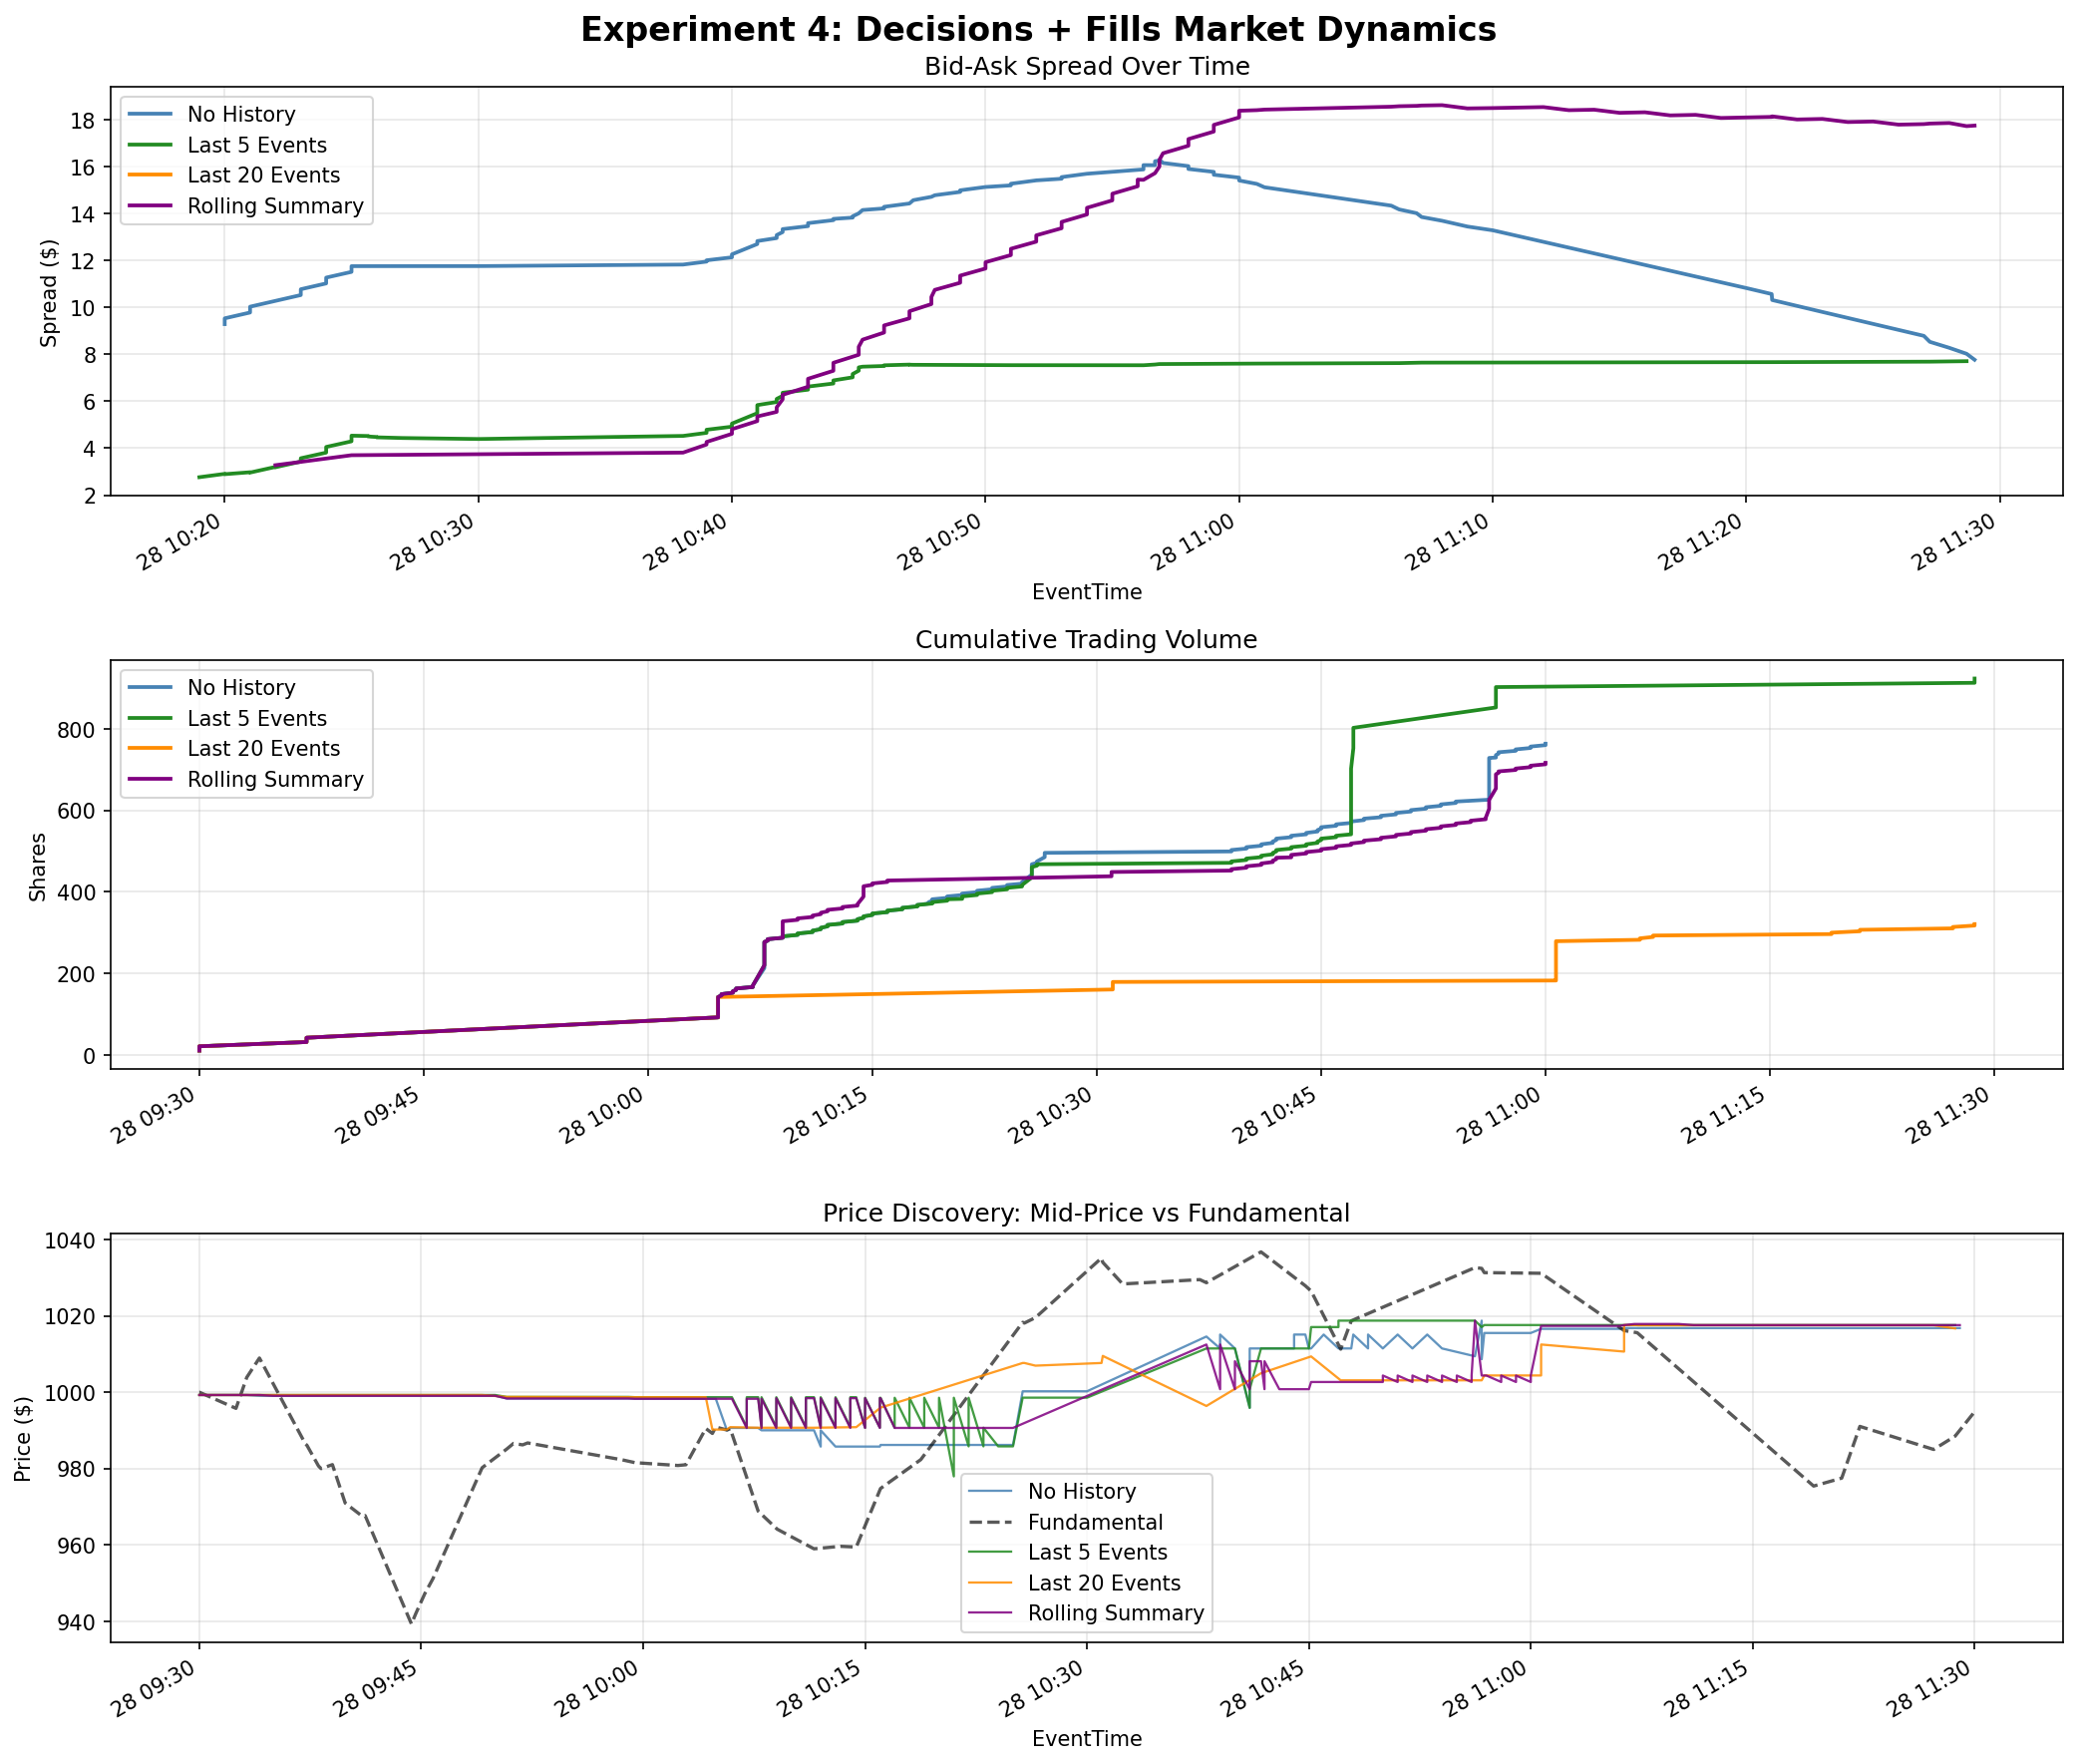
\includegraphics[width=0.92\linewidth]{exp4_decisions_fills_analysis.png}
\caption{Experiment 4 decisions-plus-fills diagnostic: spread, cumulative volume, and mid-price versus fundamental value.}
\label{fig:exp4-fills}
\end{figure}

\begin{table}[H]
\centering
\caption{Experiment 4 memory ablation summary}
\label{tab:exp4}
\begin{tabular}{llrrrrr}
\toprule
Run & Arm & PnL & Rank & Orders & Fills & Mean spread \\
\midrule
Decision Only & No History & \$476.88 & 3 & 100 & 5 & \$8.24 \\
Decision Only & Last 5 Events & \$4,098.52 & 1 & 119 & 10 & \$9.75 \\
Decision Only & Last 20 Events & \$4,098.52 & 1 & 119 & 15 & \$3.32 \\
Decision Only & Rolling Summary & \$3,042.80 & 1 & 119 & 8 & \$7.15 \\
Reasoning JSON & No History & \(-\$226.35\) & 7 & 118 & 10 & \$8.40 \\
Reasoning JSON & Last 5 Events & \$3,109.48 & 1 & 119 & 14 & \$8.54 \\
Reasoning JSON & Last 20 Events & \$6,004.31 & 1 & 117 & 15 & \$3.18 \\
Reasoning JSON & Rolling Summary & \$3,354.64 & 1 & 119 & 7 & \$7.26 \\
Decisions + Fills & No History & \$1,104.53 & 3 & 108 & 4 & \$8.70 \\
Decisions + Fills & Last 5 Events & \$2,478.41 & 1 & 81 & 12 & \$5.21 \\
Decisions + Fills & Last 20 Events & \$387.66 & 2 & 7 & 1 & \$4.77 \\
Decisions + Fills & Rolling Summary & \$4,576.82 & 1 & 119 & 10 & \$10.43 \\
\bottomrule
\end{tabular}
\end{table}

Under the clean decision-only baseline, all memory arms are profitable. No History earns only \$476.88, while Last 5 Events and Last 20 Events both earn \$4,098.52. Rolling Summary also performs well at \$3,042.80. This suggests that memory improves the agent's order placement, even though it does not make the model more selective about trading.

The reasoning diagnostic produces the best single outcome: Reasoning JSON with Last 20 Events earns \$6,004.31. However, reasoning is not uniformly better because the Reasoning JSON No History condition loses money. This reinforces the lesson from Experiment 3: prompt features and memory features interact, so they must not be mixed when estimating the causal effect of memory alone.

The decisions-plus-fills diagnostic shows that successful-trade memory helps most when compressed. Rolling Summary with fills earns \$4,576.82, the best result in that variant. In contrast, raw Last 20 Events with fills submits only 7 orders and earns \$387.66, suggesting that a long raw mixed memory can become distracting or overly restrictive. Across variants, the model remains buy-biased and rarely uses memory to reduce trading frequency. Memory changes the quality and execution profile of trades more than it changes the decision to trade.

The price-discovery panels show that better LLM PnL does not necessarily imply cleaner convergence to the fundamental value. Some high-PnL memory arms coincide with tight spreads or high executed volume, but the mid-price can still move in discrete steps and remain loosely coupled to the fundamental process. Thus, Experiment 4 currently supports a distinction between agent-level profitability and market-level price efficiency: memory can help the LLM earn more without proving that it improves equilibrium tracking.

\subsection{Cross-Experiment Interpretation}

The first four experiments reveal a consistent progression. A naive LLM trader is destabilizing and unprofitable. Prompt structure can convert the same local model from a poor trader into a marginally competitive one, but only when the prompt reduces ambiguity and grounds decisions in explicit state values. Memory can further improve outcomes, but only when its representation is compatible with the prompt. Raw additional context is not automatically useful; compact summaries and evidence-grounded reasoning appear safer for a 4B model under a small context and latency budget.

The preliminary results also highlight an important behavioral failure mode: the LLM almost always trades. Neither reasoning nor memory reliably induces deliberate holding. Future experiments should therefore consider explicit hold incentives or risk penalties if the goal is to study selective participation rather than order-price calibration.

\subsection{Caveats and Immediate Next Steps}

These results remain single-seed or diagnostic. Before publication, the main arms should be repeated across at least 10 seeds. Price-versus-equilibrium should be quantified with a tracking-error measure such as RMSE between mid-price and fundamental value. The next experimental priorities are Experiment 5, which isolates information access, and Experiment 6, which introduces controlled decision latency.

\section{Expected Contributions}

This project is expected to contribute:

\begin{enumerate}
    \item A reproducible benchmark for a small, locally hosted open-source LLM as a CDA trading agent evaluated against adaptive ABIDES benchmarks.
    \item A factor-by-factor account of which design choices, including prompt, memory, information, and latency, drive spread behavior, price efficiency, and PnL.
    \item Evidence on whether LLM agents improve or degrade price efficiency while changing liquidity relative to an adaptive benchmark.
    \item A controlled test of communication-induced coordination between same-side LLM agents, measured through spread widening and seller-side PnL.
\end{enumerate}

\section{Risks and Limitations}

\textbf{Model capacity.} A 4B model may produce malformed outputs or weak reasoning. The experiments treat this as an object of study rather than only an implementation problem.

\textbf{Latency confound.} Local inference latency interacts with the event-driven simulator. Experiment 6 is designed to measure this directly.

\textbf{External validity.} Simulated CDAs abstract away many real-market features. Claims are scoped to the ABIDES environment.

\textbf{Single-model scope.} Using Gemma 3 4B isolates design effects but limits cross-model generalization. Multi-model replication remains future work.

\textbf{Seed replication.} The completed results are not yet replicated across enough seeds for statistical claims.

\section{Conclusion}

The project has progressed from environment validation to LLM-specific behavioral diagnosis. Experiments 1 and 2 show that the simulation pipeline works and that a naive local LLM trader can substantially degrade market quality while losing money. Experiment 3 shows that prompt form matters: unstructured reasoning is harmful, structured reasoning improves compliance, and evidence grounding produces the best prompt-only result. Experiment 4 shows that memory can improve PnL, but only when treated as an independent experimental feature and represented in a form the model can use.

The remaining work is to replicate the completed experiments across seeds and complete the information-access, latency, shock-response, and communication experiments. Until then, Section 6 remains preliminary by design.

\begin{thebibliography}{9}

\bibitem{agrawal2025}
K. Agrawal, V. Teo, J. J. Vazquez, S. Kunnavakkam, V. Srikanth, and A. Liu, ``Evaluating LLM Agent Collusion in Double Auctions,'' arXiv preprint arXiv:2507.01413, 2025.

\bibitem{abides2020}
D. Byrd, M. Hybinette, and T. H. Balch, ``ABIDES: Towards High-Fidelity Multi-Agent Market Simulation,'' in \emph{ACM SIGSIM PADS}, arXiv:1904.12066, 2020.

\bibitem{cliff2018}
D. Cliff, ``BSE: A Minimal Simulation of a Limit-Order-Book Stock Exchange,'' arXiv preprint arXiv:1809.06027, 2018.

\bibitem{gjerstad1998}
S. Gjerstad and J. Dickhaut, ``Price Formation in Double Auctions,'' \emph{Games and Economic Behavior}, vol. 22, no. 1, pp. 1--29, 1998.

\bibitem{gode1993}
D. K. Gode and S. Sunder, ``Allocative Efficiency of Markets with Zero-Intelligence Traders,'' \emph{Journal of Political Economy}, vol. 101, no. 1, pp. 119--137, 1993.

\bibitem{lopezlira2025}
A. Lopez-Lira, ``Can Large Language Models Trade? Testing Financial Theories with LLM Agents in Market Simulations,'' arXiv preprint arXiv:2504.10789, 2025.

\bibitem{pymarketsim2024}
C. Mascioli et al., ``PyMarketSim: A market-simulation framework for continuous double-auction markets,'' in \emph{ICAIF}, 2024.

\bibitem{smith1962}
V. L. Smith, ``An Experimental Study of Competitive Market Behavior,'' \emph{Journal of Political Economy}, vol. 70, no. 2, pp. 111--137, 1962.

\end{thebibliography}

\end{document}
